%%\documentclass[ignorenonframetext]{beamer}
%\documentclass[11pt, a4paper]{article}
%\usepackage{graphicx, color}
%\usepackage{beamerarticle}
%
%\mode<article>
%{
%	\usepackage{fancyhdr}
%	\usepackage{pgf}
%	\usepackage{pifont}
%	\usepackage[colorlinks,
%	pdfauthor="CREEM Univ. of St. Andrews",
%	pdftitle="Guidance workshop statistical modelling Marine Scotland"]{hyperref}
%	\pagestyle{fancy}
%	\renewcommand{\headrulewidth}{0.5pt}
%	\renewcommand{\footrulewidth}{0.5pt}
%	\cfoot{\thepage}
%	\lfoot{University of St. Andrews}
%	%\rfoot{Statistical Modelling Workshop}
%	\renewcommand{\familydefault}{\sfdefault}
%	
%	%\newcommand{\hidden}[1]{{#1}}
%	\newcommand{\hidden}[1]{\textcolor{blue}{#1}}
%
%}
%
%\mode<presentation>
%{
%    \setbeamertemplate{navigation symbols}{}
%	\usetheme [height=0.3in] {Rochester}
%	\usefonttheme{structurebold}
%	\usecolortheme{seagull}
%	\beamersetuncovermixins{\opaqueness<1>{25}}{\opaqueness<2->{15}}
%} 
%
%\usepackage{epsf,graphics,graphicx,fancyhdr,color,amsmath, amssymb}
%
%\parskip 0.1 in
%% ~~~~~~~~~~~~~~~~~~~~~~~~~~~~~~~
%%% maxwidth is the original width if it is less than linewidth
%%% otherwise use linewidth (to make sure the graphics do not exceed the margin)
%\makeatletter
%\def\maxwidth{ %
%  \ifdim\Gin@nat@width>\linewidth
%    \linewidth
%  \else
%    \Gin@nat@width
%  \fi
%}
%\makeatother
%
%\definecolor{fgcolor}{rgb}{0.2, 0.2, 0.2}
%\newcommand{\hlnumber}[1]{\textcolor[rgb]{0,0,0}{#1}}%
%\newcommand{\hlfunctioncall}[1]{\textcolor[rgb]{0.501960784313725,0,0.329411764705882}{\textbf{#1}}}%
%\newcommand{\hlstring}[1]{\textcolor[rgb]{0.6,0.6,1}{#1}}%
%\newcommand{\hlkeyword}[1]{\textcolor[rgb]{0,0,0}{\textbf{#1}}}%
%\newcommand{\hlargument}[1]{\textcolor[rgb]{0.690196078431373,0.250980392156863,0.0196078431372549}{#1}}%
%\newcommand{\hlcomment}[1]{\textcolor[rgb]{0.180392156862745,0.6,0.341176470588235}{#1}}%
%\newcommand{\hlroxygencomment}[1]{\textcolor[rgb]{0.43921568627451,0.47843137254902,0.701960784313725}{#1}}%
%\newcommand{\hlformalargs}[1]{\textcolor[rgb]{0.690196078431373,0.250980392156863,0.0196078431372549}{#1}}%
%\newcommand{\hleqformalargs}[1]{\textcolor[rgb]{0.690196078431373,0.250980392156863,0.0196078431372549}{#1}}%
%\newcommand{\hlassignement}[1]{\textcolor[rgb]{0,0,0}{\textbf{#1}}}%
%\newcommand{\hlpackage}[1]{\textcolor[rgb]{0.588235294117647,0.709803921568627,0.145098039215686}{#1}}%
%\newcommand{\hlslot}[1]{\textit{#1}}%
%\newcommand{\hlsymbol}[1]{\textcolor[rgb]{0,0,0}{#1}}%
%\newcommand{\hlprompt}[1]{\textcolor[rgb]{0.2,0.2,0.2}{#1}}%
%
%\usepackage{framed}
%\makeatletter
%\newenvironment{kframe}{%
% \def\at@end@of@kframe{}%
% \ifinner\ifhmode%
%  \def\at@end@of@kframe{\end{minipage}}%
%  \begin{minipage}{\columnwidth}%
% \fi\fi%
% \def\FrameCommand##1{\hskip\@totalleftmargin \hskip-\fboxsep
% \colorbox{shadecolor}{##1}\hskip-\fboxsep
%     % There is no \\@totalrightmargin, so:
%     \hskip-\linewidth \hskip-\@totalleftmargin \hskip\columnwidth}%
% \MakeFramed {\advance\hsize-\width
%   \@totalleftmargin\z@ \linewidth\hsize
%   \@setminipage}}%
% {\par\unskip\endMakeFramed%
% \at@end@of@kframe}
%\makeatother
%
%\definecolor{shadecolor}{rgb}{.97, .97, .97}
%\definecolor{messagecolor}{rgb}{0, 0, 0}
%\definecolor{warningcolor}{rgb}{1, 0, 1}
%\definecolor{errorcolor}{rgb}{1, 0, 0}
%\newenvironment{knitrout}{}{} % an empty environment to be redefined in TeX
%
%\usepackage{alltt}
%\setbeamertemplate{navigation symbols}{}
%\usetheme [height=0.25in] {Rochester}
%\usefonttheme{structurebold}
%\usecolortheme{seagull}
%\beamersetuncovermixins{\opaqueness<1>{25}}{\opaqueness<2->{15}}
%
%\usepackage{setspace}
%\usepackage{natbib}
%\usepackage{bm}
%\usepackage{url}
%\usepackage{subfig}
%\usepackage[font=footnotesize, labelfont=bf]{caption}
%
%\setbeamertemplate{caption}[numbered]
%
%%~~~~~~~~~~~~~~~~~~~~~~~~~~~~~~~~~~~~
%\begin{document}
%
%
\begin{titlepage}


\begin{center}
\vspace* {0.70 in}

\noindent\makebox[\linewidth]{\rule{\paperwidth}{0.4pt}}

\huge{Using the {\tt MRSea} Package (v0.1.2)}\\[0.5 cm]
%\Large{University of St. Andrews}\\
\Large{Statistical Modelling of bird and cetacean distributions in offshore renewables development areas}\\
\vspace{0.3 in}
\today

\noindent\makebox[\linewidth]{\rule{\paperwidth}{0.4pt}}


\vspace{1 in}
\Large{Lindesay Scott-Hayward}\\
\Large{Cornelia Oedekoven}\\
\Large{Monique Mackenzie}\\
\Large{Cameron Walker}\\
\Large{Eric Rexstad}\\[0.5 cm]


\vspace{1.6 in}
\begin{center}
\large{This review constitutes work carried out at the Centre for Research into Ecological and Environmental Modelling (CREEM) at the University of St. Andrews, performed under contract for Marine Scotland (SB9 (CR/2012/05)).}
\end{center}


\thispagestyle{empty}

\end{center}

\end{titlepage}

%
%\title{Statistical modelling of animal distributions in offshore renewables development areas}  
%\author{Centre for Research into \\
% Ecological and Environmental Modelling \\
% University of St. Andrews}
%\date{10 September 2013} 
%\begin{frame}
%\titlepage
%\end{frame}
%
%\begin{frame}\frametitle{Table of contents}\tableofcontents
%\end{frame} 

\chapter{Offshore Worked Example}
%~~~~~~~~~~~~~~~~~~~~~~~~~~~~~~~~~~~~~~~~~
%~~~~~~~~~~~~~~~~~~~~~~~~~~~~~~~~~~~~~~~~~~~
\section{Introduction}

This document takes you through the process of fitting a detection function model to distance sampling data and then fitting spatial models using the CReSS method in a GEE framework with SALSA for model selection.  The last section uses the fitted count model to make predictions across the entire study area - including those areas not surveyed - which we use to draw inference from our study. We use simulated segmented line transect data as our case study. The type of impact was a redistribution of animals within the study area. 
%~~~~~~~~~~~~~~~~~~~~~~~~~~~~~~~~~~~~~~~~~
%~~~~~~~~~~~~~~~~~~~~~~~~~~~~~~~~~~~~~~~~~~~
\section{Two-Stage Modelling of Distance Sampling Data}
\subsection{A brief introduction}
For distance sampling data, we recognise that the number of observed animals along transect lines is a result of two underlying processes: 
\begin{enumerate}
\item{Observation process: not all animals in the covered area are detected}
\item{Distribution of animals}
\end{enumerate}

\noindent These two processes are modelled in two stages. In a first stage we fit a detection function to the observed perpendicular distances from the transect to the detection. This detection function enables us to estimate the average detection probability in the covered area used to adjust observed counts for imperfect detection. We describe how to use the code from this package to fit detection functions in section \ref{ss:fittingdetectionfunctions}, how to select between contending models in section \ref{ss:modelselection} and to assess models in section \ref{ss:goodnessoffit}. \\
These adjusted counts are then modelled in a second stage count model using covariates that relate to how animals distribute themselves in the study area. \\
Interest generally lies in the count model, while the detection function model involves nuisance parameters that need to be taken into account by estimating the average detection probability in the covered area in a first stage detection model. \\
We do this for two main reasons:
\begin{itemize}
\item{The observed counts need to be adjusted for imperfect detection}
\item{To estimate the uncertainty associated with the observation process
}
\end{itemize}
The latter requires non-parametric bootstrapping for propagation of uncertainty from the first-state detection model into count model. Non-parametric bootstrapping for distance sampling data is explained in section \ref{ss:bootstrap}.
%~~~~~~~~~~~~~~~~~~~~~~~~~~~~~~~~~~~~~~~~~
%~~~~~~~~~~~~~~~~~~~~~~~~~~~~~~~~~~~~~~~~~~~

\section{Preparing to conduct an analysis with MRSea} 
Before we start, we load the {\tt MRSea} package and its dependencies. 
This may require installing the following packages if they are not already installed on your computer: 
\begin{itemize}
\item mrds, lawstat, car, mvtnorm, splines, geepack, ggplot2, calibrate, Matrix and fields.
\end{itemize}
After installing these packages, the following command will load package {\tt MRSea} and these packages into the active workspace. 
\begin{knitrout}\footnotesize
\definecolor{shadecolor}{rgb}{0.969, 0.969, 0.969}\color{fgcolor}
\begin{kframe}
\hlfunctioncall{require}(\hlstring{MRSea})
\end{kframe}
\end{knitrout}

To find what data sets are available for testing use the following command:\\
\begin{knitrout}\footnotesize
\definecolor{shadecolor}{rgb}{0.969, 0.969, 0.969}\color{fgcolor}
\begin{kframe}
\hlfunctioncall{data}(package=\hlstring{"MRSea"})
\end{kframe}
\begin{verbatim}
Data sets in package ‘MRSea’:

dis.data.de                 Line transect data with decrease post-impact
dis.data.no                 Line transect data with no post-impact consequence
dis.data.re                 Line transect data with redistribution post-impact
knotgrid.ns                 Knot grid data for nearshore example
knotgrid.off                Knot grid data for offshore example
ns.data.de                  Nearshore data with decrease post-impact
ns.data.no                  Nearshore data with no effect of impact
ns.data.re                  Nearshore data with redistribution post-impact
ns.predict.data.de          Prediction grid data for nearshore post-impact decrease
ns.predict.data.no          Prediction grid data for nearshore no post-impact consequence
ns.predict.data.re          Prediction grid data for nearshore post-impact redistribution
predict.data.de             Prediction grid data for post-impact decrease
predict.data.no             Prediction grid data for no post-impact consequence
predict.data.re             Prediction grid data for post-impact redistribution
\end{verbatim}
\end{knitrout}
%~~~~~~~~~~~~~~~~~~~~~~~~~~~~~~~~~~~~~~~~~
%~~~~~~~~~~~~~~~~~~~~~~~~~~~~~~~~~~~~~~~~~~~
\section{Data Requirements} 
Distance sampling data generally contains three types of information on the observed animals. Our example consists of segmented line transect data, i.e.\ line transect data where the lines were divided into segments. The three types of information on the observed animals are: 
\begin{enumerate}
\item Observed perpendicular distances for each detection
\item Total number of detections for each segment
\item Cluster size for each detection
\end{enumerate}
We begin with a data frame that contains all the information necessary. Columns can be divided into three levels, the observation, segment and transect level. 
\subsection{Data requirements: columns}
\textbf{Observation level}\\
\begin{itemize}
\item{\textit{object} Object number, no repeats allowed} \\
\item{\textit{distance} Perpendicular distance in metres for line transects, required if distances were recorded as exact}\\
%\item{\textit{distbegin} Left cutpoint of distance interval in metres, required if data were collected in distance intervals (see function \textit{which.bin} for adding this column)} \\
%\item{\textit{distend} Right cutpoint of distance interval in metres, required if data were collected in distance intervals (see function \textit{which.bin} for adding this column)}\\
%\item{\textit{size} If the detections are clustered objects, the data frame should contain the observed number of individuals in the cluster} \\
\item{Optional covariates for detection function modelling}\\
\end{itemize}

\noindent \textbf{Segment level}\\
\begin{itemize}
\item{\textit{segment.id} Segment ids, no repeats of the same segment ids for different transects or different visits to the same segments allowed}\\
\item{\textit{segment.label} Segment label} \\
\item{\textit{length} Length of segment in km}\\
\item{Optional covariates for detection function and count modelling}\\
\end{itemize}

\noindent \textbf{Transect level}\\
\begin{itemize}
\item{\textit{transect.id} Transect id}\\
\item{Optional covariates for detection function and count modelling}\\
\end{itemize}

\subsection{Data Requirements: rows} 
\begin{itemize}
\item{One record for each detection}
\item{One record for each visit to a segment in case no detections were made}
\end{itemize}
\noindent We note that information entered at the respective levels is assumed to be the same for each entry for the respective \textit{object, segment.id} or \textit{transect.id}. Information entered at the observation level may vary. Information entered at the segment level needs to be the same for all records with the same \textit{segment.id}. Information entered at the transect level needs to be the same for all records with the same \textit{transect.id}. \\
To illustrate we load the data. 

\begin{knitrout}\scriptsize
\definecolor{shadecolor}{rgb}{0.969, 0.969, 0.969}\color{fgcolor}\begin{kframe}
\begin{alltt}
\hlcomment{# Loading the data}
\hlfunctioncall{data}(\hlstring{dis.data.re})
\hlfunctioncall{head}(dis.data.re)
\end{alltt}
\begin{verbatim}
  transect.id transect.label season impact segment.id
1           1              1      1      0          1
2           1              1      1      0          2
3           1              1      1      0          3
4           1              1      1      0          4
5           1              1      1      0          5
6           1              1      1      0          6
  segment.label length  x.pos   y.pos   depth object distance
1           1-1  0.306 656250 6043750 -27.359     NA       NA
2           1-2  0.500 656250 6044250 -27.561     NA       NA
3           1-3  0.500 656250 6044750 -28.608     NA       NA
4           1-4  0.500 656250 6045250 -27.999     NA       NA
5           1-5  0.500 656250 6045750 -27.519     NA       NA
6           1-6  0.500 656250 6046250 -27.223     NA       NA
\end{verbatim}
\end{kframe}
\end{knitrout}
\noindent We note that the first six records, contain the information for six different \textit{segment.id}s where no detections were made. Hence, we have one record for each visit to a segment and \textit{NA}'s in the columns pertaining to the observation level. 

\begin{knitrout}\footnotesize
\definecolor{shadecolor}{rgb}{0.969, 0.969, 0.969}\color{fgcolor}\begin{kframe}
\begin{verbatim}
dis.data.re[214:218,]
    transect.id transect.label season impact segment.id
214           6              6      1      0        183
215           6              6      1      0        183
216           6              6      1      0        183
217           6              6      1      0        184
218           6              6      1      0        185
    segment.label length  x.pos   y.pos   depth object  distance
214          6-22    0.5 666250 6046250 -11.302     41  74.13493
215          6-22    0.5 666250 6046250 -11.302     42 154.87536
216          6-22    0.5 666250 6046250 -11.302     43 192.34939
217          6-23    0.5 666250 6046750  -9.283     NA        NA
218          6-24    0.5 666250 6047250  -6.870     NA        NA
\end{verbatim}
\end{kframe}
\end{knitrout}
\noindent From these records we can see that for \textit{segment.id} 183, three detections were made, hence we have three records, one for each detection. \\

%~~~~~~~~~~~~~~~~~~~~~~~~~~~~~~~~~~~~~~~~~
%~~~~~~~~~~~~~~~~~~~~~~~~~~~~~~~~~~~~~~~~~~~


\section{Distance Analysis}
\subsection{Fitting detection functions}
\label{ss:fittingdetectionfunctions}
We begin by fitting a half-normal detection function to our data. We will consider other models and compare the relative fit of these models using AIC. 
\begin{knitrout}\footnotesize
\definecolor{shadecolor}{rgb}{0.969, 0.969, 0.969}\color{fgcolor}
\begin{kframe}
\begin{alltt}
\hlcomment{# Fitting a half-normal detection function}
result <- \hlfunctioncall{ddf}(dsmodel=~mcds(key=\hlstring{"hn"}, formula=~1), 
     data = dis.data.re, method="ds", meta.data=list(width=250))
\end{alltt}
\end{kframe}
\end{knitrout}
\begin{block}{The ddf function}
A summary of the object created by \textit{ddf} can be obtained using: 
\end{block}
\begin{knitrout}\scriptsize
\definecolor{shadecolor}{rgb}{0.969, 0.969, 0.969}\color{fgcolor}
\begin{kframe}
\noindent
\hlfunctioncall{summary}(result)
\begin{verbatim}
Summary for ds object 
Number of observations :  2373 
Distance range         :  0  -  250 
AIC                    :  25446.68 

Detection function:
 Half-normal key function 

Detection function parameters 
Scale Coefficients:  
            estimate         se
(Intercept) 4.754715 0.02068034

                        Estimate           SE         CV
Average p              0.5639511  0.009623902 0.01706513
N in covered region 4207.8115128 91.704527557 0.02179388
\end{verbatim}
\end{kframe}
\end{knitrout}
\begin{block}{Conclusion}
We conclude that the average detection probability in the covered region was 0.56 with a coefficient of variation of 1.7\%. 
\end{block}

\noindent We can also use the ddf object for plotting our detection function with a histogram of the detections. 
\begin{knitrout}\footnotesize
\definecolor{shadecolor}{rgb}{0.969, 0.969, 0.969}\color{fgcolor}
\begin{kframe}
\begin{alltt}
\hlfunctioncall{plot}(result,showpoints=F,breaks=seq(0,250,10),
     main=\hlstring{"All data combined"})
\end{alltt}
\end{kframe}
\end{knitrout}
\begin{figure}[h]
  \centering
 % \subfloat{
  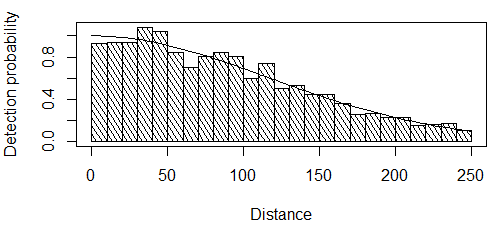
\includegraphics[width=11cm]{HN_alldatacombined.png}
%  }
 % \hfill
\caption{Half-normal detection function}
\label{fig:HN_all}
\end{figure}

\subsection{Model Selection}
\label{ss:modelselection}
More detection models can be fitted to determine if any of these provide a better relative fit to the data. 
\begin{knitrout}\footnotesize
\definecolor{shadecolor}{rgb}{0.969, 0.969, 0.969}\color{fgcolor}
\begin{kframe}
\begin{alltt}
\hlcomment{# Using a hazard-rate detection function}
result.hr <- \hlfunctioncall{ddf}(dsmodel=~mcds(key=\hlstring{"hr"}, formula=~1), 
     data = dis.data.re, method="ds", meta.data=list(width=250))
\hlcomment{# Using a half-normal function with \textit{impact} as a covariate}
result.imp <- \hlfunctioncall{ddf}(dsmodel=~mcds(key=\hlstring{"hn"}, formula=~1+impact), 
     data = dis.data.re, method="ds", meta.data=list(width=250))
\end{alltt}
\end{kframe}
\end{knitrout}
\begin{block}{The ddf function}
Changing the key function from half-normal to hazard-rate is done using the argument \textit{key}.\\
Adding covariates to the model is done by altering the argument \textit{formula}.\\
\end{block}

\noindent \textbf{Using minimum AIC for model selection}\\
The AIC value for each detection model can be printed using the \textit{summary} function. These may also be extracted from the \textit{ddf} object in this manner: 
\begin{knitrout}\footnotesize
\definecolor{shadecolor}{rgb}{0.969, 0.969, 0.969}\color{fgcolor}
\begin{kframe}
\begin{alltt}
\hlcomment{# Half-normal model}
result$criterion 
[1] 25446.68
\hlcomment{# Hazard-rate model}
result.hr$criterion 
[1] 25454.93
\hlcomment{# Half-normal model with \textit{impact} as a covariate}
result.imp$criterion 
[1] 25448.21
\end{alltt}
\end{kframe}
\end{knitrout}
\begin{block}{Conclusion}
The half-normal model has the lowest AIC. Results are slightly ambiguous as the difference in AIC is less than 2 when compared to the \textit{impact}-model. 
\end{block}

\subsection{Goodness of fit}
There are several goodness of fit tests for detection function models included in the {\tt mrds} package. We show how to use them in this section. 
\label{ss:goodnessoffit}
\frametitle{The $\chi^2$ - Test}
\noindent A chi-sqare test is performed by the \textit{ddf.gof} function. The object this function returns contains various results that can be extracted individually: 
\begin{knitrout}\footnotesize
\definecolor{shadecolor}{rgb}{0.969, 0.969, 0.969}\color{fgcolor}
\begin{kframe}
\begin{alltt}
fit.test <- \hlfunctioncall{ddf.gof}(result)\\
\hlcomment{# Chi-square statistic, p-value and degrees of freedom}
fit.test$chisquare$chi1$chisq
[1] 41.64964
fit.test$chisquare$chi1$p
[1] 0.6931487
fit.test$chisquare$chi1$df
[1] 47
\end{alltt}
\end{kframe}
\end{knitrout}
\begin{block}{Conclusion}
The large p-value provides no evidence against the null hypothesis that the model fits the data. 
\end{block}

\frametitle{QQ-plot}
\noindent We may wish to assess the model fit using a QQ-plot. This plot allows identifying potential problems related to our distance data such as rounding of distances or overdispersed distance data. 
\begin{block}{The qqplot.ddf function}
This function plots the observed distribution of the distance data vs.\ the fitted distribution of the distance data. \\
In addition, it performs the Kolmogorov-Smirnov and Cram\'{e}r-von Mises tests. 
\end{block}
\begin{knitrout}\footnotesize
\definecolor{shadecolor}{rgb}{0.969, 0.969, 0.969}\color{fgcolor}
\begin{kframe}\begin{alltt}
qq.result <- \hlfunctioncall{qqplot.ddf}(result)
\end{alltt}\end{kframe}\end{knitrout}
\begin{figure}[ht]
  \centering
  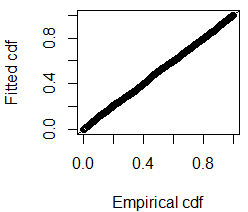
\includegraphics[width=7cm]{qqresult.png}
\caption{QQ plot for half-normal detection function fitted to our data}
\label{fig:QQ_HN_all}
\end{figure}
\begin{block}{Conclusion}
The points lie on the diagonal line, we conclude that the fit of our half-normal model is adequate. 
\end{block}

\frametitle{K-S and C-v-M tests}
\noindent The Kolmogorov-Smirnov and Cram\'{e}r-von Mises test results are extracted using:
\begin{knitrout}\footnotesize
\definecolor{shadecolor}{rgb}{0.969, 0.969, 0.969}\color{fgcolor}
\begin{kframe}
\begin{alltt}
\hlcomment{# Kolmogorov-Smirnov statistic and p-value}
qq.result$ks$Dn
[1] 0.01503729
qq.result$ks$p
[1] 0.6566394
\hlcomment{# Cram\'{e}r-von Mises statistic and p-value}
qq.result$CvM$W
[1] 0.07091705
qq.result$CvM$p
[1] 0.7459479
\end{alltt}
\end{kframe}
\end{knitrout}
\begin{block}{Conclusion}
Both p-values are large, hence we conclude that our model fits the data. 
\end{block}

%~~~~~~~~~~~~~~~~~~~~~~~~~~~~~~~~~~~~~~~~~
%~~~~~~~~~~~~~~~~~~~~~~~~~~~~~~~~~~~~~~~~~~~

\subsection{Adjusting counts for imperfect detection}
\noindent We use the \textit{create.NHAT} function to add two new columns to our distance data: \textit{NHAT} and \textit{area}. \textit{NHAT} is the estimated number of animals (as opposed to the observed number of animals) for each detection and \textit{area} is the size of the covered area for the respective \textit{segment.id}.\\
\begin{knitrout}\footnotesize
\definecolor{shadecolor}{rgb}{0.969, 0.969, 0.969}\color{fgcolor}
\begin{kframe}
\begin{alltt}
dis.data <- \hlfunctioncall{create.NHAT}(dis.data,result)
\end{alltt}
\end{kframe}
\end{knitrout}
\begin{block}{The create.NHAT function}
We inflate our number of detected animals by dividing the size of each detection by its probability of being detected which was estimated by the \textit{ddf} function.\\
We also calculate the covered area in km$^2$ for each \textit{segment.id} by multiplying the length of the segment by twice the truncation distance (for two-sided transects). 
\end{block}

\subsection{Creating Count Data from Distance Data}
\noindent We create a new data frame in which we sum the \textit{NHATs} for each \textit{segment.id} and discard the columns from the observation layer because the observations themselves are not modelled with the count modelling to follow. 
\begin{knitrout}\footnotesize
\definecolor{shadecolor}{rgb}{0.969, 0.969, 0.969}\color{fgcolor}
\begin{kframe}
\begin{alltt}
count.data <- \hlfunctioncall{create.count.data}(dis.data)
\end{alltt}
\end{kframe}
\end{knitrout}
\begin{block}{The create.count.data function}
We aggregate the data by \textit{segment.id}. This reduces the number of records in the count data to one for each visit to a segment. 
\end{block}


%~~~~~~~~~~~~~~~~~~~~~~~~~~~~~~~~~~~~~~~~~
%~~~~~~~~~~~~~~~~~~~~~~~~~~~~~~~~~~~~~~~~~~~
\section{Introduction to Spatial Modelling} 
\begin{frame}
\frametitle{Introduction} 

\begin{block}{Aim}
Produce a density surface map along with estimates of uncertainty and identify significant effects of an impact (e.g.\ offshore renewable installation)
\end{block}

The following sections details the following:

\begin{enumerate}
  \item model fitting 
  \item checking diagnostics
  \item making predictions and inference
\end{enumerate}

\bigskip

Note: This example assumes that any distance sampling analysis has taken place and begin with the adjusted counts in each segment.  
\end{frame}


%~~~~~~~~~~~~~~~~~~~~~~~~~~~~~~~~~~~~~~~~~
%~~~~~~~~~~~~~~~~~~~~~~~~~~~~~~~~~~~~~~~~~~~

\section{Loading the Data}
\begin{frame}[fragile]
\frametitle{Loading the Data}
Either continue from the previous section with {\tt count.data} or, load {\tt count.data} if it was savedt.\\

\noindent \textbf{Requirements}:\\

\noindent The coordinates must be labelled {\tt x.pos} and {\tt y.pos}, there must be a column for segment area, labelled {\tt area} and the estimated counts from the detection process must be labelled {\tt NHAT}. Both are manufactured by \textit{create.NHAT}.
\begin{knitrout}\footnotesize
\definecolor{shadecolor}{rgb}{0.969, 0.969, 0.969}\color{fgcolor}\begin{kframe}
\begin{alltt}
\hlcomment{# make effort column segment length * 0.5 (width of}
\hlcomment{# transect) - twice truncation distance}
\hlfunctioncall{attach}(count.data)
\hlfunctioncall{head}(count.data)
\end{alltt}
\begin{verbatim}
  transect.id transect.label season impact segment.id
1           1              1      1      0          1
2           1              1      1      0          2
3           1              1      1      0          3
4           1              1      1      0          4
5           1              1      1      0          5
6           1              1      1      0          6
  segment.label length  x.pos   y.pos  depth  area NHAT
1           1-1  0.306 656250 6043750 -27.36 0.153    0
2           1-2  0.500 656250 6044250 -27.56 0.250    0
3           1-3  0.500 656250 6044750 -28.61 0.250    0
4           1-4  0.500 656250 6045250 -28.00 0.250    0
5           1-5  0.500 656250 6045750 -27.52 0.250    0
6           1-6  0.500 656250 6046250 -27.22 0.250    0
\end{verbatim}
\end{kframe}
\end{knitrout}

\end{frame}

\begin{frame}[fragile]
\frametitle{Exploratory Data Analysis}
First we assess the data inputs for the modelling process.
\begin{itemize}
\item Check estimates from distance sampling process
\item Check for unusual covariate values
\item Identify possible relationships between covariates and the response (animal counts)
\end{itemize}

\begin{figure}[h]
\centering
  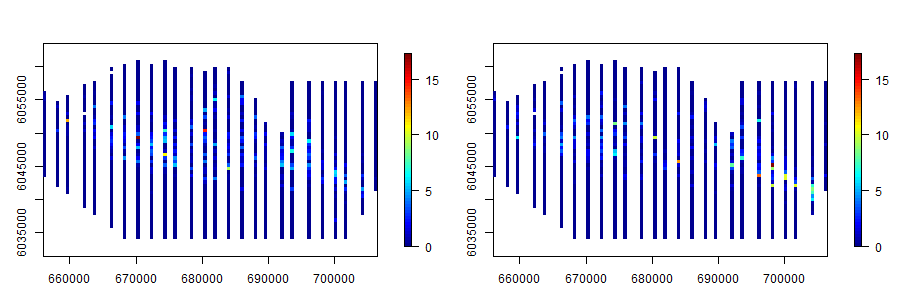
\includegraphics[width=9cm]{nhats.png}
\caption{Estimated bird counts before (left) and after (right) an impact event.  Each cell is 0.5 km$^2$ and the colour represents mean animal counts across four seasons.}
\label{fig:rawnhats}
\end{figure}
\end{frame}


\begin{frame}
\frametitle{}
Assessing the relationships of available covariates and our response (animal counts).
\end{frame}

\begin{frame}
\frametitle{}
\begin{figure}[h]
  \centering
  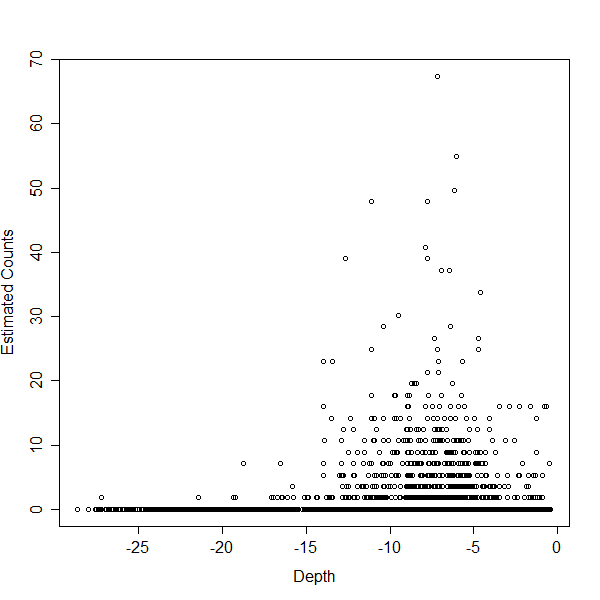
\includegraphics[width=7cm]{depth.png}
\caption{Plot of depth against the estimated bird counts.}
\label{fig:exploratory1}
\end{figure}
\end{frame}

\begin{frame}
\frametitle{}
\begin{figure}[h]
  \centering
  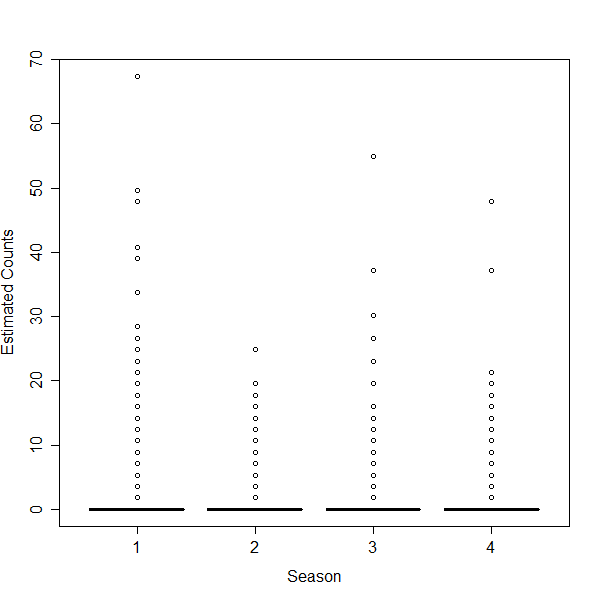
\includegraphics[width=7cm]{season.png}
\caption{Plot of Season against the estimated bird counts.}
\label{fig:exploratory2}
\end{figure}
\end{frame}

\begin{frame}
\frametitle{}
\begin{figure}[h]
  \centering
  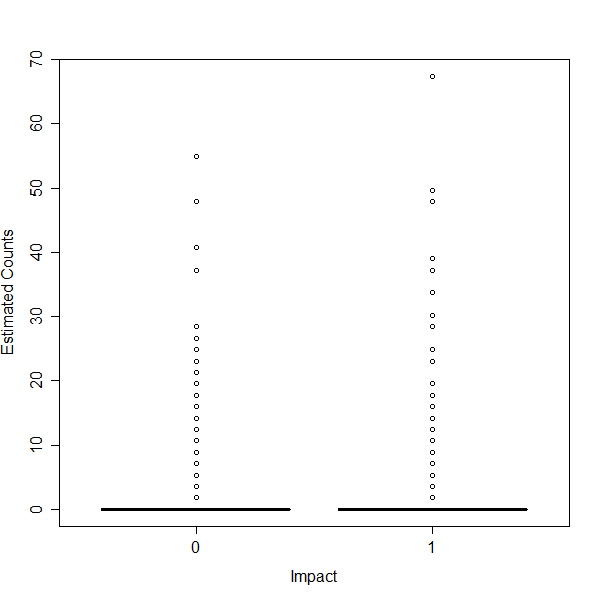
\includegraphics[width=7cm]{impact.png}
\caption{Plot of Impact against the estimated bird counts. Zero is pre impact and one is post impact.}
\label{fig:exploratory3}
\end{figure}
\end{frame}

\begin{frame}
%\frametitle{EDA}
\begin{itemize}
\item Birds were seen predominantly in shallow waters (Figure \ref{fig:exploratory1}).
\item Few birds were seen in waters deeper than 15m.  
\item Non-linear relationship between depth and bird counts.  
\item Difficult to identify any relationship between season/impact and bird counts due to the large number of zeros in the data (Figures \ref{fig:exploratory2} \&  \ref{fig:exploratory3}).
\end{itemize}
\end{frame}
%~~~~~~~~~~~~~~~~~~~~~~~~~~~~~~~~~~~~~~~~~
%~~~~~~~~~~~~~~~~~~~~~~~~~~~~~~~~~~~~~~~~~~~

\begin{frame}[fragile]
\frametitle{Checking for Collinear variables}
\begin{block}{Variance Inflation Factors (VIFs)}
To assess collinearity between covariates and tell us by how much the standard error is inflated by the other variables in the model.
\end{block}

\begin{itemize}
\item Generalised VIFs (GVIFs) are calculated, because the covariates have more than one degree of freedom, and adjusted (GVIF$_{\textrm{adj}}$ = GVIF$^{1/2*Df}$) for the number of degrees of freedom.
\item GVIF$_{\textrm{adj}}$ gives us the decrease in precision of estimation due to collinearity (equivalent to $\sqrt{VIF}$). 
\item For example, a GVIF$_{\textrm{adj}}$ of 2 means that the confidence intervals are twice as wide as they would be for uncorrelated predictors.
\end{itemize}
\end{frame}

\subsection{Checking for Co-linearity}
\begin{frame}[fragile]
%\frametitle{Checking for Co-linearity}
\begin{knitrout}\footnotesize
\definecolor{shadecolor}{rgb}{0.969, 0.969, 0.969}\color{fgcolor}\begin{kframe}
\begin{alltt}
fullModel.linear <- \hlfunctioncall{glm}(NHAT ~ \hlfunctioncall{as.factor}(season) + \hlfunctioncall{as.factor}(impact) + 
    depth + x.pos + y.pos, family = poisson, data =count.data)
\hlfunctioncall{vif}(fullModel.linear)
\end{alltt}
\begin{verbatim}
                   GVIF Df GVIF^(1/(2*Df))
as.factor(season) 1.000  3           1.000
as.factor(impact) 1.000  1           1.000
depth             4.745  1           2.178
x.pos             1.494  1           1.222
y.pos             5.309  1           2.304
\end{verbatim}
\end{kframe}
\end{knitrout}

\begin{knitrout}\footnotesize
\definecolor{shadecolor}{rgb}{0.969, 0.969, 0.969}\color{fgcolor}\begin{kframe}
\begin{verbatim}
[1] "Maximum VIF is: 2.3"
\end{verbatim}
\end{kframe}
\end{knitrout}
\begin{block}{}
The large values for {\tt depth} and {\tt y.pos} suggests the confidence intervals are twice as wide as they should be for these covariates. One could be removed, however, {\tt y.pos} will not enter our model linearly.  Suggest check again when spatial smooth fitted
\end{block}
\end{frame}

\begin{frame}[fragile]
\frametitle{Checking factor covariates}
Each level of a factor based covariate must have some non-zero entries, otherwise the will be problems in the model fitting process 
\begin{knitrout}\footnotesize
\definecolor{shadecolor}{rgb}{0.969, 0.969, 0.969}\color{fgcolor}\begin{kframe}
\begin{alltt}
\hlcomment{# check all factor levels have counts}
\hlfunctioncall{checkfactorlevelcounts}(factorlist=\hlfunctioncall{c}(\hlstring{"season"}, \hlstring{"impact"}), count.data, 
                      count.data$NHAT)
\end{alltt}
\begin{verbatim}
[1] "season will be fitted as a factor variable; 
there are non-zero counts for all levels"
[1] "impact will be fitted as a factor variable; 
there are non-zero counts for all levels"
\end{verbatim}
\end{kframe}
\end{knitrout}
\begin{block}{}
Conclusion: season and impact are fine for use in the model.
\end{block}
\end{frame}
%~~~~~~~~~~~~~~~~~~~~~~~~~~~~~~~~~~~~~~~~~
%~~~~~~~~~~~~~~~~~~~~~~~~~~~~~~~~~~~~~~~~~~~
\section{Fitting a Model}

\begin{frame}[fragile]
\frametitle{}
Here we are going to fit a GEE-CReSS model with SALSA for knot selection. Recap:
\begin{block}{Generalised Estimating Equations (GEE)}
Framework to allow for correlated errors.
\end{block}

\begin{block}{Complex Region Spatial Smoother (CReSS)}
Flexible spatial smoothing method.
\end{block}

\begin{block}{Spatially Adaptive Local Smoothing Algorithm (SALSA)}
Automated knot selection procedure for both one-dimensional (e.g. depth) and two-dimensional (e.g. the x, y plane) covariates.  The knots are sources of flexibility in the surface that can raise or lower the surface.
\end{block}
\end{frame}


\subsection{Fitting a Smooth Term}

\begin{frame}[fragile]
\frametitle{A smooth of depth}

Construct an object ({\tt splineParams}) that contains the information required by SALSA for adaptive knot placement.
\begin{itemize}
\item Each covariate considered smooth is a list entry in {\tt splineParams}
\item The list contains the covariate name, data, initial knot location (one knot at the mean), the boundary knots (greatest range of prediction data and {\tt count.data}) and the degree of the smooth.
\item Note:  The smooth one dimensional covariates appear in the {\tt splineParams} object starting at slot {\tt [[2]]}. Slot {\tt [[1]]} is reserved for the spatial term.
\end{itemize}

\begin{knitrout}\footnotesize
\definecolor{shadecolor}{rgb}{0.969, 0.969, 0.969}\color{fgcolor}\begin{kframe}
\begin{alltt}
\hlcomment{# load prediction data}
\hlfunctioncall{data}(predict.data.re)

\hlcomment{# make splineParams object}
splineParams<-\hlfunctioncall{makesplineParams}(data=count.data, varlist=\hlfunctioncall{c}(\hlstring{'depth'}),
         predictionData=predict.data.re)
\hlfunctioncall{str}(splineParams)
\begin{verbatim}
List of 2
 $ : list()
 $ :List of 5
  ..$ covar      : chr "depth"
  ..$ explanatory: num [1:9232] -27.4 -27.6 -28.6 -28 -27.5 ...
  ..$ knots      : num -12.4
  ..$ bd         : num [1:2] -28.6 -0.2
  ..$ degree     : num 2
\end{verbatim}
\end{alltt}
\end{kframe}
\end{knitrout}

\begin{knitrout}\footnotesize
\definecolor{shadecolor}{rgb}{0.969, 0.969, 0.969}\color{fgcolor}\begin{kframe}
\begin{alltt}
fullModel <- \hlfunctioncall{glm}(NHAT ~ \hlfunctioncall{as.factor}(season) + \hlfunctioncall{as.factor}(impact) + 
    \hlfunctioncall{bs}(depth, knots = splineParams[[2]]$knots) + x.pos + y.pos, family = 
quasipoisson,  data = count.data)
\end{alltt}
\end{kframe}
\end{knitrout}
\end{frame}

\subsection{Checking for Correlation}

\begin{frame}[fragile]
\frametitle{Checking for Correlation}
We fit a model containing all covariates of interest ({\tt fullModel} above) and carry out some \textbf{runs tests} to check for \textbf{correlated residuals} (model assumes uncorrelated residuals).

\begin{block}{Runs Test}
This is a test for randomness and allows us to determine if we have correlation in our model residuals. We will see a large $p$-value (H$_0$: uncorrelated residuals) and good mixing of the profile plot if there is no correlation.
\end{block}

\end{frame}

\begin{frame}[fragile]
\frametitle{}
\noindent The {\tt runs.test} function is in the {\tt lawstat} library
\begin{knitrout}\footnotesize
\definecolor{shadecolor}{rgb}{0.969, 0.969, 0.969}\color{fgcolor}\begin{kframe}
\begin{alltt}
\hlfunctioncall{runs.test}(\hlfunctioncall{residuals}(fullModel, type = \hlstring{"pearson"}), 
alternative = \hlfunctioncall{c}(\hlstring{"two.sided"}))
\end{alltt}
\begin{verbatim}
	Runs Test - Two sided
data:  residuals(fullModel, type = "pearson") 
Standardized Runs Statistic = -67.28, p-value <
2.2e-16
\end{verbatim}
\end{kframe}
\end{knitrout}

\begin{itemize}
\item The small $p$-value ($p << 0.05$) indicates that there is an issue with correlation in the residuals
\item The test statistic is negative, which indicates that there are fewer runs of residuals than would be expected if there were un-correlated residuals.  We have positive correlation.
\item This result is also shown on the runs profile plot (Figure \ref{fig:runs1}).
\end{itemize}
\end{frame}

\vspace{1cm}

\begin{frame}[fragile]
\frametitle{Plotting runs profile}
\begin{knitrout}\footnotesize
\definecolor{shadecolor}{rgb}{0.969, 0.969, 0.969}\color{fgcolor}\begin{kframe}
\begin{alltt}
\hlfunctioncall{plotRunsProfile}(fullModel,  varlist = \hlfunctioncall{c}(\hlstring{"depth"}))
\end{alltt}
\begin{verbatim}
[1] "Calculating runs test and plotting profile"
\end{verbatim}
\end{kframe}
\end{knitrout}

\begin{figure}[h]
  \centering
 \subfloat[]{
  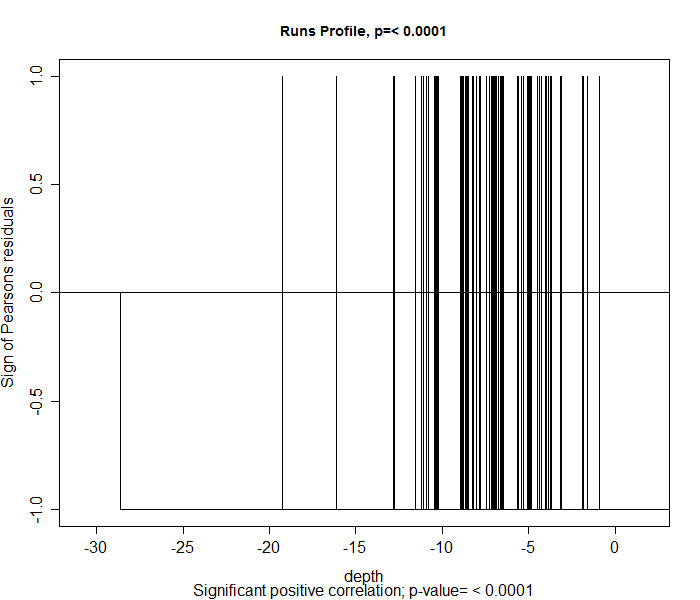
\includegraphics[width=6cm]{RunsProfile_depth_glmk1.png}
\label{fig:sub:runs1a}
}	
  \hfill
  \subfloat[]{
        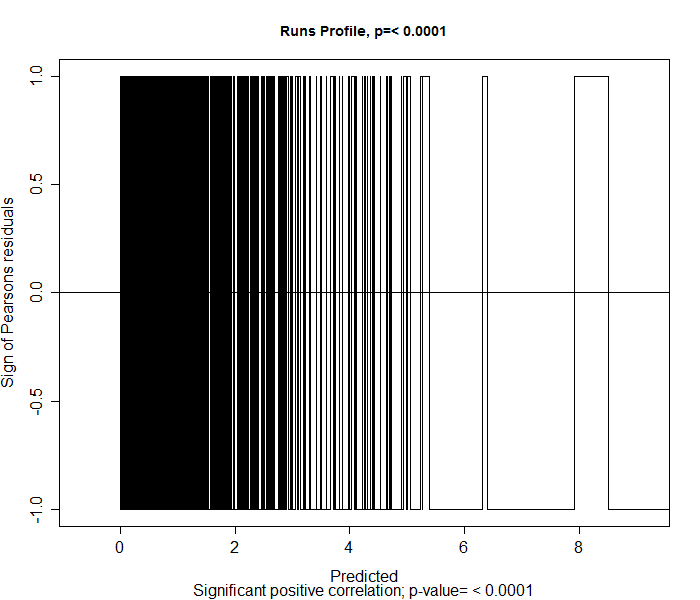
\includegraphics[width=6cm]{RunsProfile_Predicted_glmk1.png}
\label{fig:sub:runs1b}
}	
  \hfill
   \subfloat[]{
      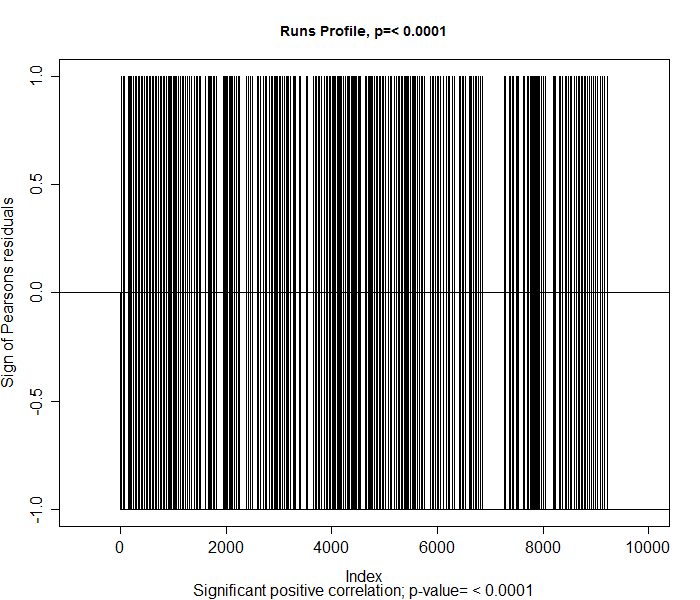
\includegraphics[width=6cm]{RunsProfile_Index_glmk1.png}
\label{fig:sub:runs1c}
}	
  \hfill
\caption{Runs profiles for residuals ordered by (a) depth, (b) predicted value and (c) temporally (by observation index). The $p$-values and text presented on each plot indicate if there is correlation present in the residuals.  The lines are the strings of sequences of positive and negative residuals.  A vertical line is the switch between a positive and negative run (or vice versa).}
\label{fig:runs1}
\end{figure}
\end{frame}

\begin{frame}
\frametitle{Checking for Correlation}
\begin{itemize}
\item Runs test and plots show an issue with correlated residuals
\item We have positive correlation in the residuals no matter how they are ordered.
%\item Depth could be modelled more appropriately according to the cumulative residual plot (the black line (our model) does not correspond well with the expected line (grey)).
\pause
\item Conclusion:  
\begin{itemize}
  \item We have correlation that must be accounted for
  %\item we might want to consider more flexibility for {\tt depth}.
\end{itemize}
\end{itemize}
\end{frame}

\begin{frame}
\frametitle{Choosing a blocking structure to model correlation.}
\begin{itemize}
\item Correlation within blocks should decline to approximately zero 
\item Between blocks residuals should be uncorrelated
\item Blocks are usually determined by the sampling design
\item Here we use the unique transect identifier: Each transect is independent but residuals may be correlated within a transect.
\item There are 26 transects repeated 8 times (4 seasons before and 4 after the impact event) giving us 208 blocks.
\end{itemize}
\end{frame}


\begin{frame}[fragile]
\frametitle{Autocorrelation function plot}
We can check the correlation declines within our blocks by plotting the autocorrelation of the model residuals by block (Figure \ref{fig:acf}).  First we must make a column in our data (if it does not already exist) that represents the blocking structure we wish to use.

\begin{knitrout}\footnotesize
\definecolor{shadecolor}{rgb}{0.969, 0.969, 0.969}\color{fgcolor}\begin{kframe}
\begin{alltt}
count.data$blockid <- \hlfunctioncall{paste}(data$transect.id, data$season, data$impact, 
    sep = \hlstring{""})
\hlfunctioncall{runACF}(count.data$blockid, fullModel, store = F)
\end{alltt}
\end{kframe}
\end{knitrout}


\begin{itemize}
\item Some blocks have little correlation, whilst others have high correlation (0.25) at a lag of 10 segments which in this case equates to a distance of 5km.
\item Correlation in all blocks declines to approximately zero, which we want to see if our blocking is appropriate
\item If the correlation in \emph{all} blocks declined very quickly to zero (after one lag) we need not model the correlation
\pause
\item Conclusion: Our blocking structure is suitable
\end{itemize}
\end{frame}

\begin{frame}[fragile]
\frametitle{Autocorrelation function plot}
\begin{figure}[h]
  \centering
  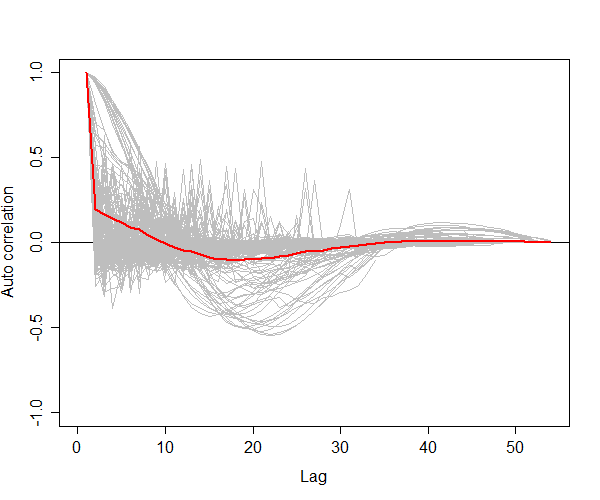
\includegraphics[width=9cm]{acfPlot.png}
\caption{Plot of the correlation in residuals for each block (grey lines).  The mean correlation at each lag is indicated in red.}
\label{fig:acf}
\end{figure}
\end{frame}



\clearpage
%~~~~~~~~~~~~~~~~~~~~~~~~~~~~~~~~~~~~~~~~~
%~~~~~~~~~~~~~~~~~~~~~~~~~~~~~~~~~~~~~~~~~~~

\subsection{Model Selection}
\begin{frame}[fragile]
\frametitle{}
Select what one-dimensional covariates to include in the model and use SALSA to determine the knot locations of those that are continuous: {\tt depth}.

\noindent We use cumulative residual plots to check for \textbf{appropriately modelled covariates}.  
\begin{itemize}
\item These plots show systematic over- or under- prediction.  
\item We expect to see good mixing (lots of peaks and troughs) and deviation from this may indicate the covariate is not modelled appropriately.
\item Figure \ref{fig:cumres1} shows cumulative residual plots from a model with depth modelled as a linear term and with one knot at the mean.
\end{itemize} 
\end{frame}

\begin{frame}[fragile]
\frametitle{Plotting Cumulative Residuals}
\begin{knitrout}\footnotesize
\definecolor{shadecolor}{rgb}{0.969, 0.969, 0.969}\color{fgcolor}\begin{kframe}
\begin{alltt}
\hlcomment{# plotting cumulative residuals for the model with depth as a smooth term}
\hlfunctioncall{plotCumRes}(fullModel, varlist= \hlfunctioncall{c}(\hlstring{"depth"}), splineParams)
\end{alltt}
\begin{verbatim}
"Calculating cumulative residuals"
\end{verbatim}
\end{kframe}
\end{knitrout}

\begin{figure}[h]
  \centering
 \subfloat[]{
  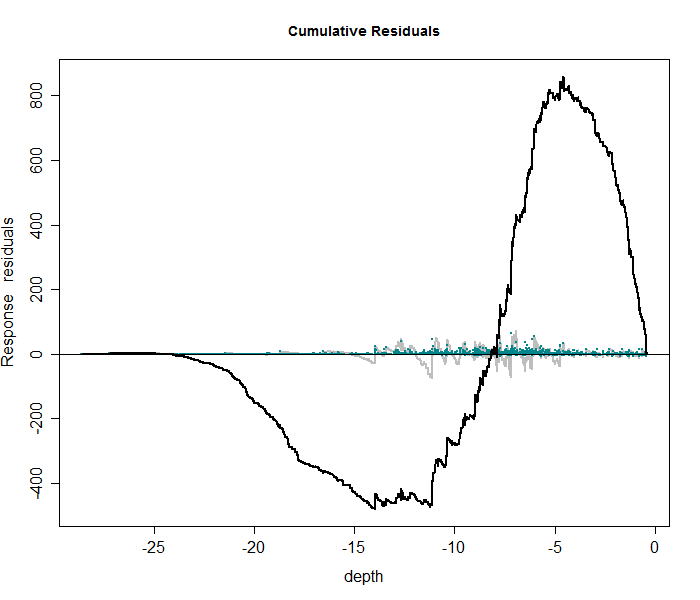
\includegraphics[width=6cm]{CumRes_depth_glm.png}
\label{fig:sub:cumres1a}
}	
  \hfill
  \subfloat[]{
        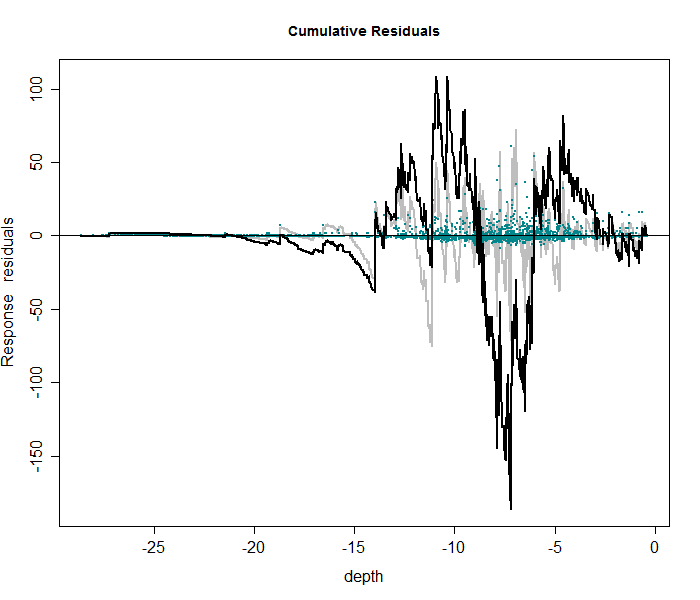
\includegraphics[width=6cm]{CumRes_depth_glmk1.png}
\label{fig:sub:cumres1b}
}	
\caption{Cumulative residual plots residuals ordered by depth. (a) depth modelled as a linear term and (b) depth modelled with one knot at the mean depth.  The blue points are the residual values, the black line represents the cumulative residuals. The grey line in the background is what we would expect the cumulative residuals to be if depth was modelled correctly.}
\label{fig:cumres1}
\end{figure}
\end{frame}

\begin{frame}
\frametitle{Cumulative Residuals}
\begin{itemize}
\item Depth as a linear term is not appropriate (Figure \ref{fig:sub:cumres1a}).
\item The black line (our model) does not correspond well with the expected line (grey) and shows systematic over prediction at deeper depths and under prediction in shallower waters.
\item Depth as a smooth term with one knot at the mean is much better but there is still some evidence of systematic over/under prediction (Figure \ref{fig:sub:cumres1b}).
\pause
\item Conclusion:  
\begin{itemize}
  \item we might want to consider more flexibility for {\tt depth} by using SALSA.
\end{itemize}
\end{itemize}
\end{frame}


\begin{frame}[fragile]
\frametitle{Setting up the model for SALSA}
\begin{itemize}
\item There must be a column called {\tt response} in the data, which is the response variable used in the initial model to be fitted.
\item The object {\tt salsa1dlist} contains parameters for the {\tt runSALSA1D} function.  
\begin{itemize}
\item {\tt fitnessMeasure}. The criterion for selecting the `best' model.  Available options: AIC, AIC$_c$, BIC, QIC$_b$.
\item {\tt minKnots\_1d}. Minimum number of knots to be tried.
\item {\tt maxKnots\_1d}. Maximum number of knots to be tried.
\item {\tt startKnots\_1d}. Starting number of knots (spaced at quantiles of the data).
\item {\tt degree}. The degree of the B-spline. Does not need to be specified if {\tt splineParams} is a parameter in {\tt runSALSA1D}.
\item {\tt maxIterations}. The exchange/improve steps will terminate after maxIterations if still running.
\item {\tt gaps}. The minimum gap between knots (in unit of measurement of explanatory).
\end{itemize}
\item The initial model contains all the factor level covariates and any covariates of interest that are not specified in the {\tt varlist} argument of {\tt runSALSA1D}.
\end{itemize}

\begin{knitrout}\footnotesize
\definecolor{shadecolor}{rgb}{0.969, 0.969, 0.969}\color{fgcolor}\begin{kframe}
\begin{alltt}
\hlcomment{# info for SALSA}
data$response <- data$NHAT

salsa1dlist <- \hlfunctioncall{list}(fitnessMeasure = \hlstring{"QICb"}, minKnots_1d = 2, 
                    maxKnots_1d = 20, startKnots_1d = 2, degree = 2, 
                    maxIterations = 10, gaps = \hlfunctioncall{c}(1))

\hlcomment{# set initial model without the spline terms in there (so}
\hlcomment{# all other non-spline terms)}
initialModel <- \hlfunctioncall{glm}(response ~ \hlfunctioncall{as.factor}(season) + \hlfunctioncall{as.factor}(impact) + 
    \hlfunctioncall{offset}(\hlfunctioncall{log}(area)), family = \hlstring{"quasipoisson"}, data = count.data)

\end{alltt}
\end{kframe}
\end{knitrout}

\begin{knitrout}\footnotesize
\definecolor{shadecolor}{rgb}{0.969, 0.969, 0.969}\color{fgcolor}\begin{kframe}
\begin{alltt}
\hlcomment{# run SALSA}
salsa1dOutput <- \hlfunctioncall{runSALSA1D}(initialModel, salsa1dlist, varlist=\hlfunctioncall{c}(\hlstring{"depth"}), 
    factorlist=\hlfunctioncall{c}(\hlstring{"Season"}, \hlstring{"Impact"}), predictData, splineParams=splineParams)
\end{alltt}
\end{kframe}
\end{knitrout}
\end{frame}

\begin{frame}[fragile]
\frametitle{}
\noindent The structure of the output: 
\begin{itemize}
\item {\tt bestModel}. The model object for the best fitted model.
\item {\tt modelFits1D}.  Each slot in the list shows the term fitted, the fit statistic resulting from that term, the knots used and finally the overall formula.  If {\tt varlist} is more than one covariate, this output shows how each covariate was retained and what knots were finalised.
\item {\tt splineParams}.  The spline parameter object is updated with the new knot numbers and locations of the covariates from {\tt varlist}.
\item {\tt fitStat}.  The fit statistic of the best model.
\end{itemize}

\begin{knitrout}\footnotesize
\definecolor{shadecolor}{rgb}{0.969, 0.969, 0.969}\color{fgcolor}\begin{kframe}
\begin{alltt}
\hlfunctioncall{str}(salsa1dOutput, max.level = 1)
\end{alltt}
\begin{verbatim}
List of 4
 $ bestModel   :List of 30
  ..- attr(*, "class")= chr [1:2] "glm" "lm"
 $ modelFits1D :List of 2
 $ splineParams:List of 2
 $ fitStat     : num 8464
\end{verbatim}
\end{kframe}
\end{knitrout}
\end{frame}

\begin{frame}[fragile]
\frametitle{}
\begin{knitrout}\footnotesize
\definecolor{shadecolor}{rgb}{0.969, 0.969, 0.969}\color{fgcolor}\begin{kframe}
\begin{alltt}
\hlcomment{# knots chosen for depth}
salsa1dOutput$splineParams[[2]]$knots
\end{alltt}
\begin{verbatim}
[1] -17.184  -7.457
\end{verbatim}
\end{kframe}
\end{knitrout}

\begin{itemize}
\item Initial model - one knot at the mean depth (-12.4m) 
\item SALSA result - two knots placed either side of the mean value
\item The result of SALSA is additional flexibility in the relationship between bird counts and depth.
\end{itemize}
\end{frame}

\begin{frame}[fragile]
\frametitle{Spatial component}
\begin{itemize}
\item Next we add a two dimensional CReSS smooth of geographic coordinates (s({\tt x.pos}, {\tt y.pos}))
\item To test for a redistribution of animals with an impact effect we fit an interaction term between the smooth of coordinates and {\tt impact}.
\item SALSA is used to determine spatially adaptive knot locations for this smooth term.
\end{itemize}
\end{frame}

\begin{frame}
\frametitle{}
\begin{block}{SALSA 2D requirements}
\begin{itemize}
\item A grid of knot locations
\item Matrix of knot to knot distances 
\item Matrix of data to knot distances
\item Vector of range parameters for CReSS (determines the range of effectiveness of each knot basis).  See \citep{ScottH2013} for more details.
\item Minimum, maximum and starting number of knots
\end{itemize}
\end{block}
The next section assumes that the knot grid has been defined. See section \ref{} for some guidance to do this.
\end{frame}

\begin{frame}[fragile]
\frametitle{Spatial component}
\begin{knitrout}\footnotesize
\definecolor{shadecolor}{rgb}{0.969, 0.969, 0.969}\color{fgcolor}\begin{kframe}
\begin{alltt}
\hlcomment{# load knotgrid (regular grid containing NA's for invalid knot }
\hlcomment{# locations (e.g. on land or outside study region))}
\hlfunctioncall{data}(knotgrid.off)
knotgrid <- knotgrid.off
\end{alltt}
\end{kframe}
\end{knitrout}

\noindent Figure \ref{fig:knotgrid} shows the locations of the data points and the locations of the knot points in {\tt knotgrid}.  The transects in this data are spaced 2km apart.  If knots were chosen at the same y-location on adjacent transects there are no data between them for support.  Therefore, we use a gap parameter of 4000m ({\tt x.pos} and {\tt y.pos} are in meters) to prevent adjacent knots.

\begin{figure}[h]
	\centering
	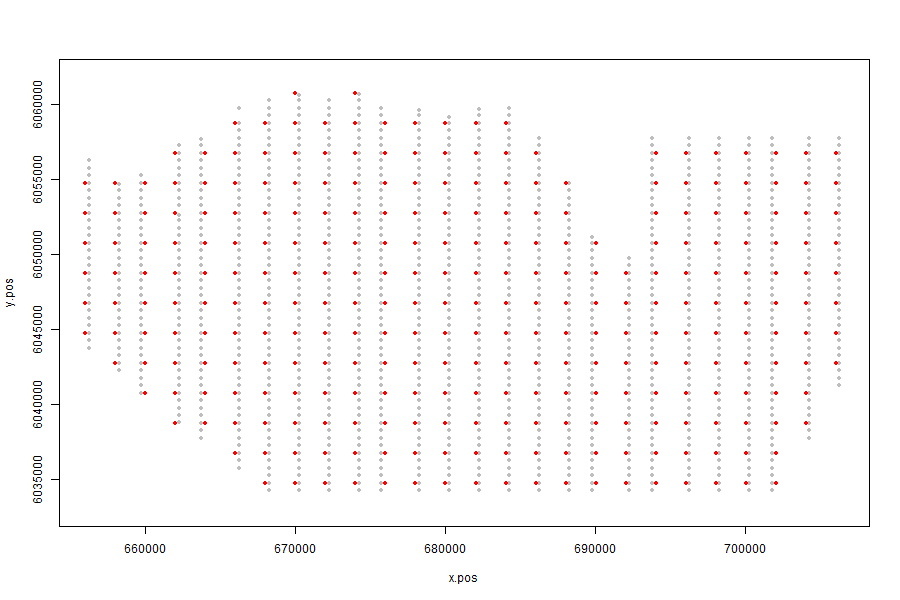
\includegraphics[width=9cm]{knotgrid.png}
	\caption{Data and knot locations.  The data is in grey and the knot locations in red.  Units are in meters.}
	\label{fig:knotgrid}
\end{figure}

\noindent The distance matrices give the distance between the data and the knots in one matrix and the second matrix is the knot to knot distances.  The function {\tt makeDists} calculates Euclidean distance. The {\tt runSALSA2D} function may also take geodesic distance matrices (as the fish swims rather than as the crow flies).  See \citet{ScottH2013} and help file for more details on geodesic distances.

\begin{knitrout}\footnotesize
\definecolor{shadecolor}{rgb}{0.969, 0.969, 0.969}\color{fgcolor}\begin{kframe}
\begin{alltt}
\hlcomment{# make distance matrices for datatoknots and knottoknots}
distMats <- \hlfunctioncall{makeDists}(\hlfunctioncall{cbind}(count.data$x.pos, count.data$y.pos), 
               \hlfunctioncall{na.omit}(knotgrid))
\hlfunctioncall{str}(distMats)
\end{alltt}
\begin{verbatim}
List of 2
 $ dataDist: num [1:9232, 1:290] 14820 15129 15448 15776 16113 ...
 $ knotDist: num [1:290, 1:290] 0 2000 4000 6000 8000 10000 ...
  ..- attr(*, "dimnames")=List of 2
  .. ..$ : chr [1:290] "7" "8" "9" "10" ...
  .. ..$ : chr [1:290] "7" "8" "9" "10" ...
\end{verbatim}
\end{kframe}
\end{knitrout}

\noindent A sequence of range parameters is required for the CReSS smooth.  
\begin{itemize}
\item The range parameter determines the influence of each knot.  
\item Small numbers are for a local influence and large ones a global influence.
\item Once knot locations are selected (using the mid value in the range sequence), SALSA selects the appropriate range parameter (from the sequence given) for each knot.
\end{itemize}
\begin{knitrout}\footnotesize
\definecolor{shadecolor}{rgb}{0.969, 0.969, 0.969}\color{fgcolor}\begin{kframe}
\begin{alltt}
\hlcomment{# choose sequence of radii}
r_seq <- \hlfunctioncall{getRadiiChoices}(numberofradii=8, distMats$dataDist)
\end{alltt}
\end{kframe}
\end{knitrout}
\end{frame}



\begin{frame}[fragile]
\frametitle{Setting up the spatial SALSA components}

\begin{itemize}
\item {\tt fitnessMeasure}. The fitness measures available are the same as for {\tt runSALSA1D}.
\item {\tt knotgrid}. $(k \times 2)$ matrix of knot coordinates.  Rows of {\tt NA}'s identify illegal knot locations
\item {\tt startKnots}. Number of space-filled knots to start with (between minKnots and maxKnots)
\item {\tt minKnots}.  Minimum number of knots to fit
\item {\tt maxKnots}.  Maximum number of knots to fit
\item {\tt r\_seq}. Sequence of range parameters for the CReSS basis.
\item {\tt gap}.  Minimum gap between knots (in unit of measurement of {\tt x.pos} and {\tt y.pos})
\item {\tt interactionTerm}. Specifies which term in the model the spatial smooth will interact with. If NULL no interaction term is fitted.
\end{itemize}



\begin{knitrout}\footnotesize
\definecolor{shadecolor}{rgb}{0.969, 0.969, 0.969}\color{fgcolor}\begin{kframe}
\begin{alltt}
\hlcomment{# make parameter set for running salsa2d}
salsa2dlist <- \hlfunctioncall{list}(fitnessMeasure = \hlstring{"QICb"}, knotgrid = knotgrid, 
    startKnots = 6, minKnots = 4, maxKnots = 20, r_seq = r_seq, 
    gap = 4000, interactionTerm = \hlstring{"as.factor(impact)"})
\end{alltt}
\end{kframe}
\end{knitrout}

\noindent The initial model is the best model from the one-dimensional SALSA results.
\begin{knitrout}\footnotesize
\definecolor{shadecolor}{rgb}{0.969, 0.969, 0.969}\color{fgcolor}\begin{kframe}
\begin{alltt}
\hlcomment{# splineParams must be an object in workspace}
\hlcomment{# update splineParams with the SALSA1D results}
splineParams <- salsa1dOutput$splineParams
salsa2dOutput_k6 <- \hlfunctioncall{runSALSA2D}(salsa1dOutput$bestModel, salsa2dlist, 
    distMats$dataDist, distMats$knotDist, 
    splineParams = splineParams)
\end{alltt}
\end{kframe}
\end{knitrout}
\end{frame}


\begin{frame}[fragile]
\frametitle{Multiple SALSA runs}

\noindent The example uses 6 starting knot locations.  There is a risk that the SALSA algorithm may get stuck in local minima or maxima and so we recommend that a variety of starting knot numbers are used.  Here we try 6, 8, 10 and 12 (Table \ref{tab:fitstats}).  \\

\noindent We use Cross-Validation (CV) as a method for selecting between models with a variety of starting knots.\\

\begin{block}{$k$-fold Cross-Validation (CV)}
\begin{itemize}
\item Method for assessing model fit where the data is split into $k$ sets and the model fitted to $k_{(-i)}$ sets and predicted to the $k_i^{th}$ set.\\
\item Mean Squared Error (MSE) is calculated for each of the $k_i$ prediction sets and a mean taken to get the CV score.\\
\item The smaller the CV score the better the model.
\end{itemize}
\end{block}

\noindent Example:
\begin{knitrout}\footnotesize
\definecolor{shadecolor}{rgb}{0.969, 0.969, 0.969}\color{fgcolor}\begin{kframe}
\begin{alltt}
count.data$foldid <- \hlfunctioncall{getCVids}(count.data, folds = 5, block = \hlstring{"blockid"})
\end{alltt}
\end{kframe}
\end{knitrout}

\begin{knitrout}\footnotesize
\definecolor{shadecolor}{rgb}{0.969, 0.969, 0.969}\color{fgcolor}\begin{kframe}
\begin{alltt}
cv1 <- \hlfunctioncall{getCV_CReSS}(count.data, salsa1dOutput$bestModel, 
           salsa1dOutput$splineParams)
\end{alltt}
\begin{verbatim}
[1] 6.087
\end{verbatim}
\end{kframe}
\end{knitrout}

\end{frame}

\begin{frame}[fragile]
\frametitle{Choosing a model}
\begin{table}[h]
\centering
\caption{Table of CV scores for a variety of starting knot numbers for the spatial smooth.}
\begin{tabular}{l|c|c|c}
\textbf{Model type} & \textbf{Start knots} & \textbf{End knots}  & \textbf{CV}\\
\hline
1D terms only & - & - & 6.0865\\
1D/2D terms & 6 & 5 & 5.6508\\
1D/2D terms & 8 & 8  & 5.8286\\
1D/2D terms & 10 & 10  & 5.7556\\
1D/2D terms & 12 & 11  & 5.7275\\
\end{tabular}
\label{tab:fitstats}
\end{table}
\end{frame}

\begin{frame}[fragile]
\frametitle{}
The best model chosen using CV score is the model that uses a spatial smooth with 6 spatial knots.
\begin{knitrout}\footnotesize
\definecolor{shadecolor}{rgb}{0.969, 0.969, 0.969}\color{fgcolor}\begin{kframe}
\begin{alltt}
\hlcomment{# having chosen the 2d interaction model, save the model object}
baseModel <- salsa2dOutput_k6$bestModel
\hlcomment{# update spline parameter object}
splineParams <- salsa2dOutput_k6$splineParams
\end{alltt}
\end{kframe}
\end{knitrout}

\end{frame}

\begin{frame}[fragile]
\frametitle{Chosen Model - recheck for collinearity}
\begin{knitrout}\footnotesize
\definecolor{shadecolor}{rgb}{0.969, 0.969, 0.969}\color{fgcolor}\begin{kframe}
\begin{alltt}
\hlfunctioncall{vif}(baseModel)
\end{alltt}
\begin{verbatim}
                                   GVIF Df GVIF^(1/(2*Df))
as.factor(season)                 1.000  3           1.000
as.factor(impact)                 2.016  1           1.420
s(depth)                          5.078  4           1.225
s(x.pos, y.pos)                   163.5  6           1.529
s(x.pos, y.pos):as.factor(impact) 96.45  6           1.4633
\end{verbatim}
\end{kframe}
\end{knitrout}
\begin{block}{}
Maximum adjusted GVIF is less than $\sqrt{5}$ (one of the cut-off's often seen in the literature) so we are happy there is no issue with collinearity.
\end{block}
\end{frame}

%~~~~~~~~~~~~~~~~~~~~~~~~~~~~~~~~~~~~~~~~~
%~~~~~~~~~~~~~~~~~~~~~~~~~~~~~~~~~~~~~~~~~~~

\subsection{Checking $p$-values}

\begin{frame}[fragile]
\frametitle{Re-assessing runs test for best model}
\begin{itemize}
\item Our best model based on CV selection is the model with the interaction term. 
\item We could also use $p$-value selection, though the model must be fitted as a GEE to model the correlation.
\end{itemize}

We must account for the correlation in our residuals, which we found earlier but should also check the current model.
\begin{knitrout}\footnotesize
\definecolor{shadecolor}{rgb}{0.969, 0.969, 0.969}\color{fgcolor}\begin{kframe}
\begin{alltt}
\hlfunctioncall{runs.test}(\hlfunctioncall{residuals}(baseModel, type = \hlstring{"pearson"}))
\end{alltt}
\begin{verbatim}
	Runs Test - Two sided
data:  residuals(baseModel, type = "pearson") 
Standardized Runs Statistic = -66.57, p-value <2.2e-16
\end{verbatim}
\end{kframe}
\end{knitrout}


\end{frame}

\begin{frame}[fragile]
\frametitle{GEE framework}
There is significant positive correlation ($p<<0.05$ and test statistic is negative) so we re-fit the model as a GEE.

\bigskip
Note: It is possible to do this at this stage as we are modelling correlation using empirical standard errors and not a specific correlation structure.

\bigskip
\noindent The current model:
\footnotesize
\begin{verbatim}
glm(formula = response ~ as.factor(season) + as.factor(impact) + 
 bs(depth, knots = splineParams[[2]]$knots, degree = 
 splineParams[[2]]$degree, Boundary.knots = splineParams[[2]]$bd) + 
 LocalRadialFunction(radiusIndices,dists,radii,aR) + 
 as.factor(impact):LocalRadialFunction(radiusIndices,dists,radii,aR) +
 offset(log(area)), family = quasipoisson, data = count.data)
\end{verbatim}
\normalsize
\end{frame}

\begin{frame}[fragile]
\begin{knitrout}\footnotesize
\definecolor{shadecolor}{rgb}{0.969, 0.969, 0.969}\color{fgcolor}\begin{kframe}
\begin{alltt}
\hlcomment{# N.B. for the GEE formula, the data must be ordered by block (which this is)}
\hlcomment{# and the blockid must be numeric}
\hlcomment{# specify parameters for local radial:}
radiusIndices <- splineParams[[1]]$radiusIndices
dists <- splineParams[[1]]$dist
radii <- splineParams[[1]]$radii
aR <- splineParams[[1]]$invInd[splineParams[[1]]$knotPos]

\hlcomment{# update model in workspace with parameters for spatial smooth (above)}
baseModel <- \hlfunctioncall{update}(baseModel, . ~ .)

\hlcomment{# Re-fit the chosen model as a GEE (based on SALSA knot placement) and}
\hlcomment{# GEE p-values}
geeModel <- \hlfunctioncall{geeglm}(\hlfunctioncall{formula}(baseModel), data = count.data, family = poisson,
                   id = blockid)
\end{alltt}
\end{kframe}
\end{knitrout}

\end{frame}

\begin{frame}[fragile]
\frametitle{Checking $p$-values}
\begin{knitrout}\footnotesize
\definecolor{shadecolor}{rgb}{0.969, 0.969, 0.969}\color{fgcolor}\begin{kframe}
\begin{alltt}
\hlcomment{# table of p-values}
\hlcomment{# specifying varlist and factorlist makes shorter variable names}
\hlfunctioncall{getPvalues}(geeModel, varlist = \hlfunctioncall{c}(\hlstring{"depth"}), factorlist = \hlfunctioncall{c}(\hlstring{"season"}, 
    \hlstring{"impact"}))
\end{alltt}
\begin{verbatim}
[1] "Getting marginal p-values"
                Variable p-value
1                 season <0.0001
2                 impact 0.5398
3                  depth <0.0001
4        s(x.pos, y.pos) <0.0001
5 s(x.pos, y.pos):impact 0.0014
\end{verbatim}
\end{kframe}
\end{knitrout}
\end{frame}


\begin{frame}[fragile]
\frametitle{Do we remove the main {\tt impact} effect?}
Either:
\begin{itemize}
\item Keep the main effect for {\tt impact} since it is part of the interaction term and is difficult to really interpret what this $p$-value actually means.\\
or\\
\item Remove the main effect for impact as it is not significant ($p>>0.05$).
\end{itemize}

\bigskip
Here we chose the first option, but below is an example of how to remove the {\tt impact} term using the {\tt update} function.
\end{frame}

\begin{frame}[fragile]
\frametitle{Removing the main {\tt impact} effect}
\begin{knitrout}\footnotesize
\definecolor{shadecolor}{rgb}{0.969, 0.969, 0.969}\color{fgcolor}\begin{kframe}
\begin{alltt}
\hlcomment{# how to remove impact}
model <- \hlfunctioncall{update}(geeModel, . ~ . - \hlfunctioncall{as.factor}(impact))
\hlcomment{# reshow p-values}
\hlfunctioncall{getPvalues}(model, varlist = \hlfunctioncall{c}(\hlstring{"depth"}), factorlist = \hlfunctioncall{c}(\hlstring{"season"}, 
    \hlstring{"impact"}))
\end{alltt}
\begin{verbatim}
[1] "Getting marginal p-values"
                Variable p-value
1                 season <0.0001
2                  depth <0.0001
3        s(x.pos, y.pos) <0.0001
4 s(x.pos, y.pos):impact <0.0001
\end{verbatim}
\end{kframe}
\end{knitrout}

\end{frame}


%~~~~~~~~~~~~~~~~~~~~~~~~~~~~~~
%~~~~~~~~~~~~~~~~~~~~~~~~~~~~~~~~~
\subsection{Assessing covariate relationships}

\begin{frame}[fragile]
\frametitle{}
\begin{block}{Partial Plots}
Visually examine the one-dimensional covariates in the model (depth, season, impact).
Check smooth/linear terms are specified correctly.
\end{block}

\begin{knitrout}\footnotesize
\definecolor{shadecolor}{rgb}{0.969, 0.969, 0.969}\color{fgcolor}\begin{kframe}
\begin{alltt}
\hlfunctioncall{runPartialPlots}(geeModel, count.data, varlist = \hlfunctioncall{c}(\hlstring{"depth"}), 
     factorlist =\hlfunctioncall{c}(\hlstring{"season"}, \hlstring{"impact"}))
\end{alltt}
\begin{verbatim}
[1] "Making partial plots"
\end{verbatim}
\end{kframe}
\end{knitrout}

\end{frame}

\begin{frame}[fragile]
\frametitle{Assessing covariate relationships}
\begin{figure}[h]
  \centering
  \subfloat[]{
    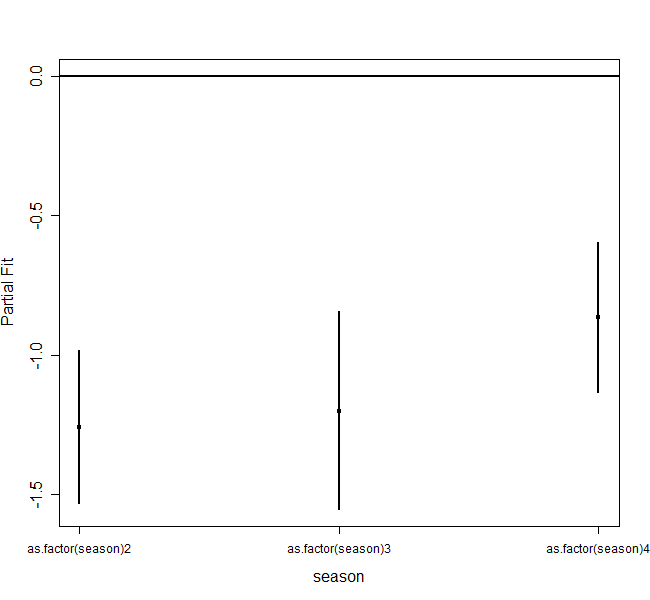
\includegraphics[width=6cm]{PartialFits1.png}
  }
  \subfloat[]{
    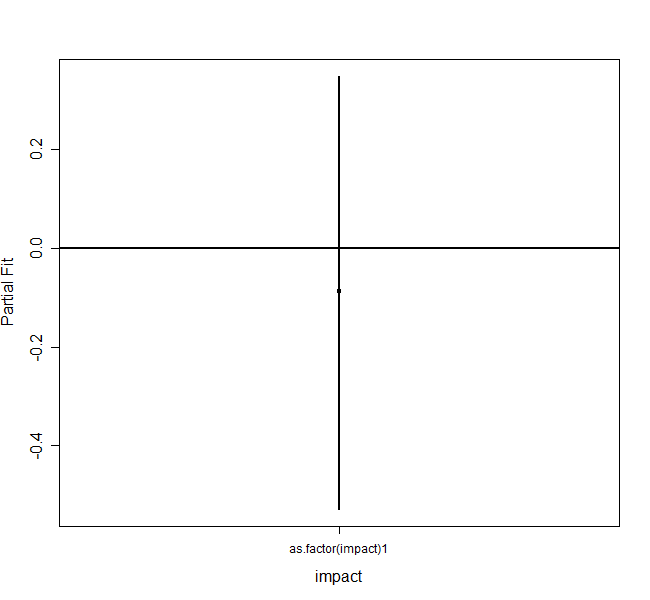
\includegraphics[width=6cm]{PartialFits2.png}
  }
  \hfill
  \subfloat[]{
    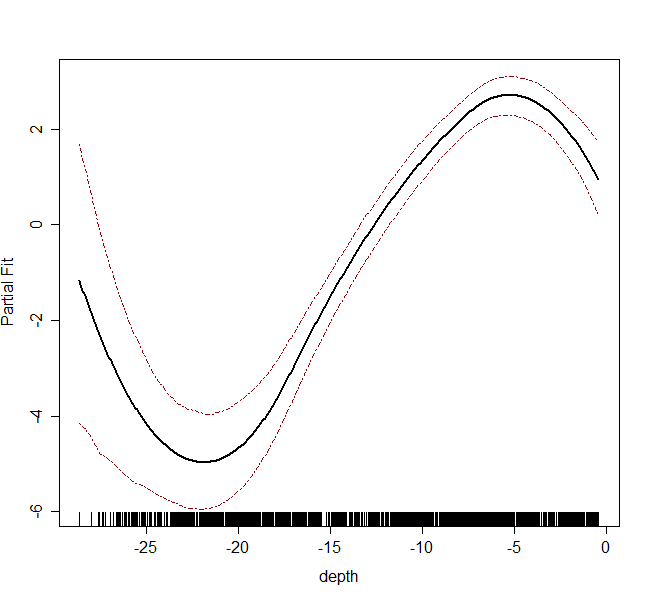
\includegraphics[width=6cm]{PartialFits3.png}
  }
  \caption{Partial plots for (a) season, (b) impact and (c) depth.}
  \label{fig:partials}
\end{figure}
\end{frame}

\begin{frame}
\frametitle{Partial Plots}
\begin{itemize}
\item Season: predictions for each of the three seasons (2, 3, 4) are, on average, of fewer animals than for the baseline (season 1).
\item GEE based confidence intervals show little difference between the three levels and the baseline level \pause
\item Impact: confirms the ANOVA $p$-value and indicates no change in bird numbers post impact.
\pause
\item Depth: a declining non-linear relationship with increased depth (fewer birds in deeper waters).
\item Most birds are estimated in waters 3-8m deep.
\item Small confidence interval indicates a precisely estimated relationship.
\end{itemize}
\pause
\bigskip
Note: if the confidence interval for depth was very wide it might indicate that depth as a linear term is more appropriate.
\end{frame}

\clearpage
%~~~~~~~~~~~~~~~~~~~~~~~~~~~~~~~~~~~~~~~~~
%~~~~~~~~~~~~~~~~~~~~~~~~~~~~~~~~~~~~~~~~~~~

\section{Diagnostics}

\begin{frame}[fragile]
\frametitle{Diagnostics}
We make multiple plots to assess the fit of our model:

\bigskip
\begin{itemize}
\item Observed vs Fitted
\item Fitted vs residuals
\item Cumulative residuals
\item Runs sequence
\item COVRATIO statistics
\item PRESS statistics
\item Raw residuals
\end{itemize}
\end{frame}

\begin{frame}[fragile]
\frametitle{Observed vs fitted Plot}

\begin{block}{Observed vs Fitted}
Indication of fit to the data.  All the values would be on the 45$^o$ line for a perfectly fitting model.    
\end{block}

\noindent The agreement between the input data and the model undergoing evaluation can be quantified using numerical measures; Marginal R-squared and Concordance Correlation. 
\end{frame}

\begin{frame}[fragile]
\frametitle{}
These measures are an output on the observed vs fitted plot. 

\begin{block}{Marginal R-squared value}
It is widely used to assess models fitted to both un-correlated and correlated data and is approximately between 0 and 1.  Values closer to 1 indicate better fit to the data.
\end{block}

\begin{block}{Concordance Correlation}
It is guaranteed to return values between zero and one.  Values closer to 1 indicate better fit to the data.
\end{block}

\begin{knitrout}\footnotesize
\definecolor{shadecolor}{rgb}{0.969, 0.969, 0.969}\color{fgcolor}\begin{kframe}
\begin{alltt}
\hlcomment{# create observed vs fitted and fitted vs residual plots}
\hlfunctioncall{runDiagnostics}(geeModel)
\end{alltt}
\begin{verbatim}
[1] "Assessing predictive power"
\end{verbatim}
\end{kframe}
\end{knitrout}

\end{frame}

\begin{frame}[fragile]
\frametitle{Observed vs fitted}
\begin{figure}[h]
  \centering
    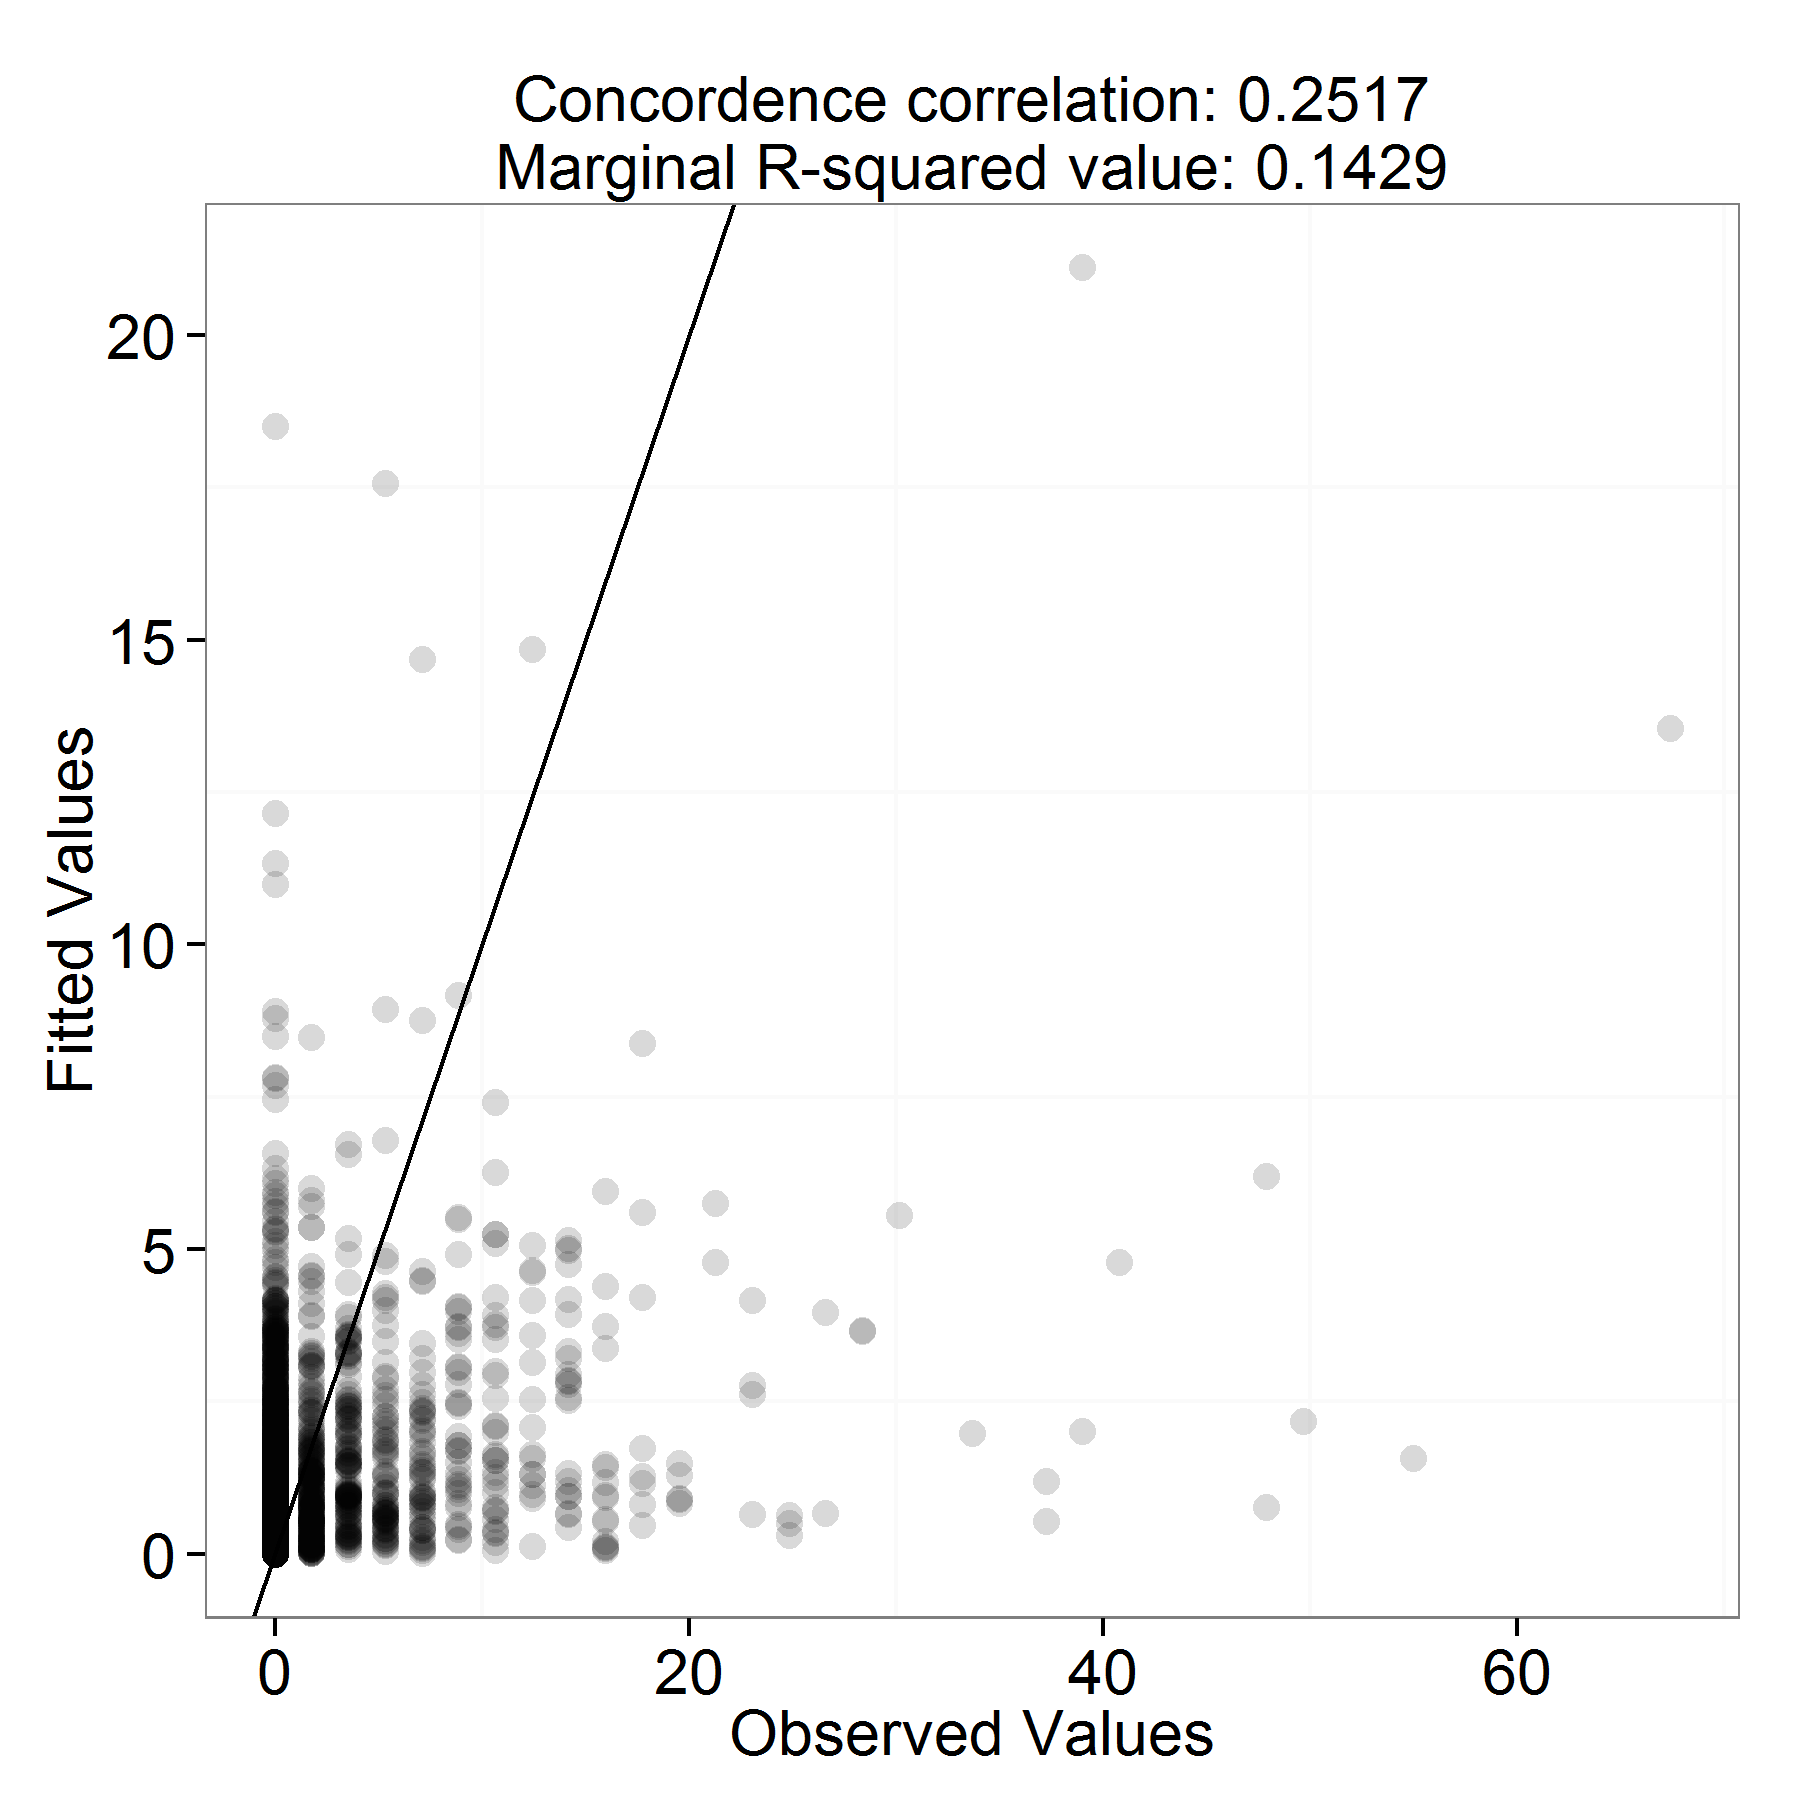
\includegraphics[width=6cm]{FitPlots_fitted.png}
  \caption{Diagnostic plots of observed vs fitted values, where the diagonal line indicates where data should lie for a perfect fit.}
  \label{fig:diagplots}
\end{figure}
\end{frame}

\begin{frame}
\frametitle{Observed vs fitted}
\begin{itemize}
\item High observed values are under-predicted
\item Observed zeros tend to be over-predicted
\item Marginal R-squared and concordance correlation are low
\pause
\bigskip
\item Conclusion: poor model fit
\end{itemize}
\end{frame}

%~~~~~~~~~~~~~~~~~~~~~~~~~~~~~~~~~~~~~~~~~~~~~~~~~~
%~~~~~~~~~~~~~~~~~~~~~~~~~~~~~~~~~~~~~~~~~~~~~~~~~~~~~

\begin{frame}[fragile]
\frametitle{Fitted values vs scaled Pearsons residuals Plot}

\begin{block}{Fitted values vs residuals}
Indication of correct mean-variance relationship (model assumption).  Expect to see no pattern in the plot.  
\end{block}

\begin{itemize}
\item For a Poisson model the size of residuals is expected to increase with increasing fitted values
\item For over-dispersed data the size of residuals increases at a faster rate than the strict Poisson relationship
\item To get a plot with an expectation of no pattern we use Pearsons residuals to account for the former and scaled these by the dispersion parameter for the latter
\item Thus we plot Fitted values against scaled Pearsons residuals
\end{itemize}
\end{frame}

\begin{frame}[fragile]
\frametitle{Fitted values vs scaled Pearsons residuals}
\begin{figure}[h]
  \centering
    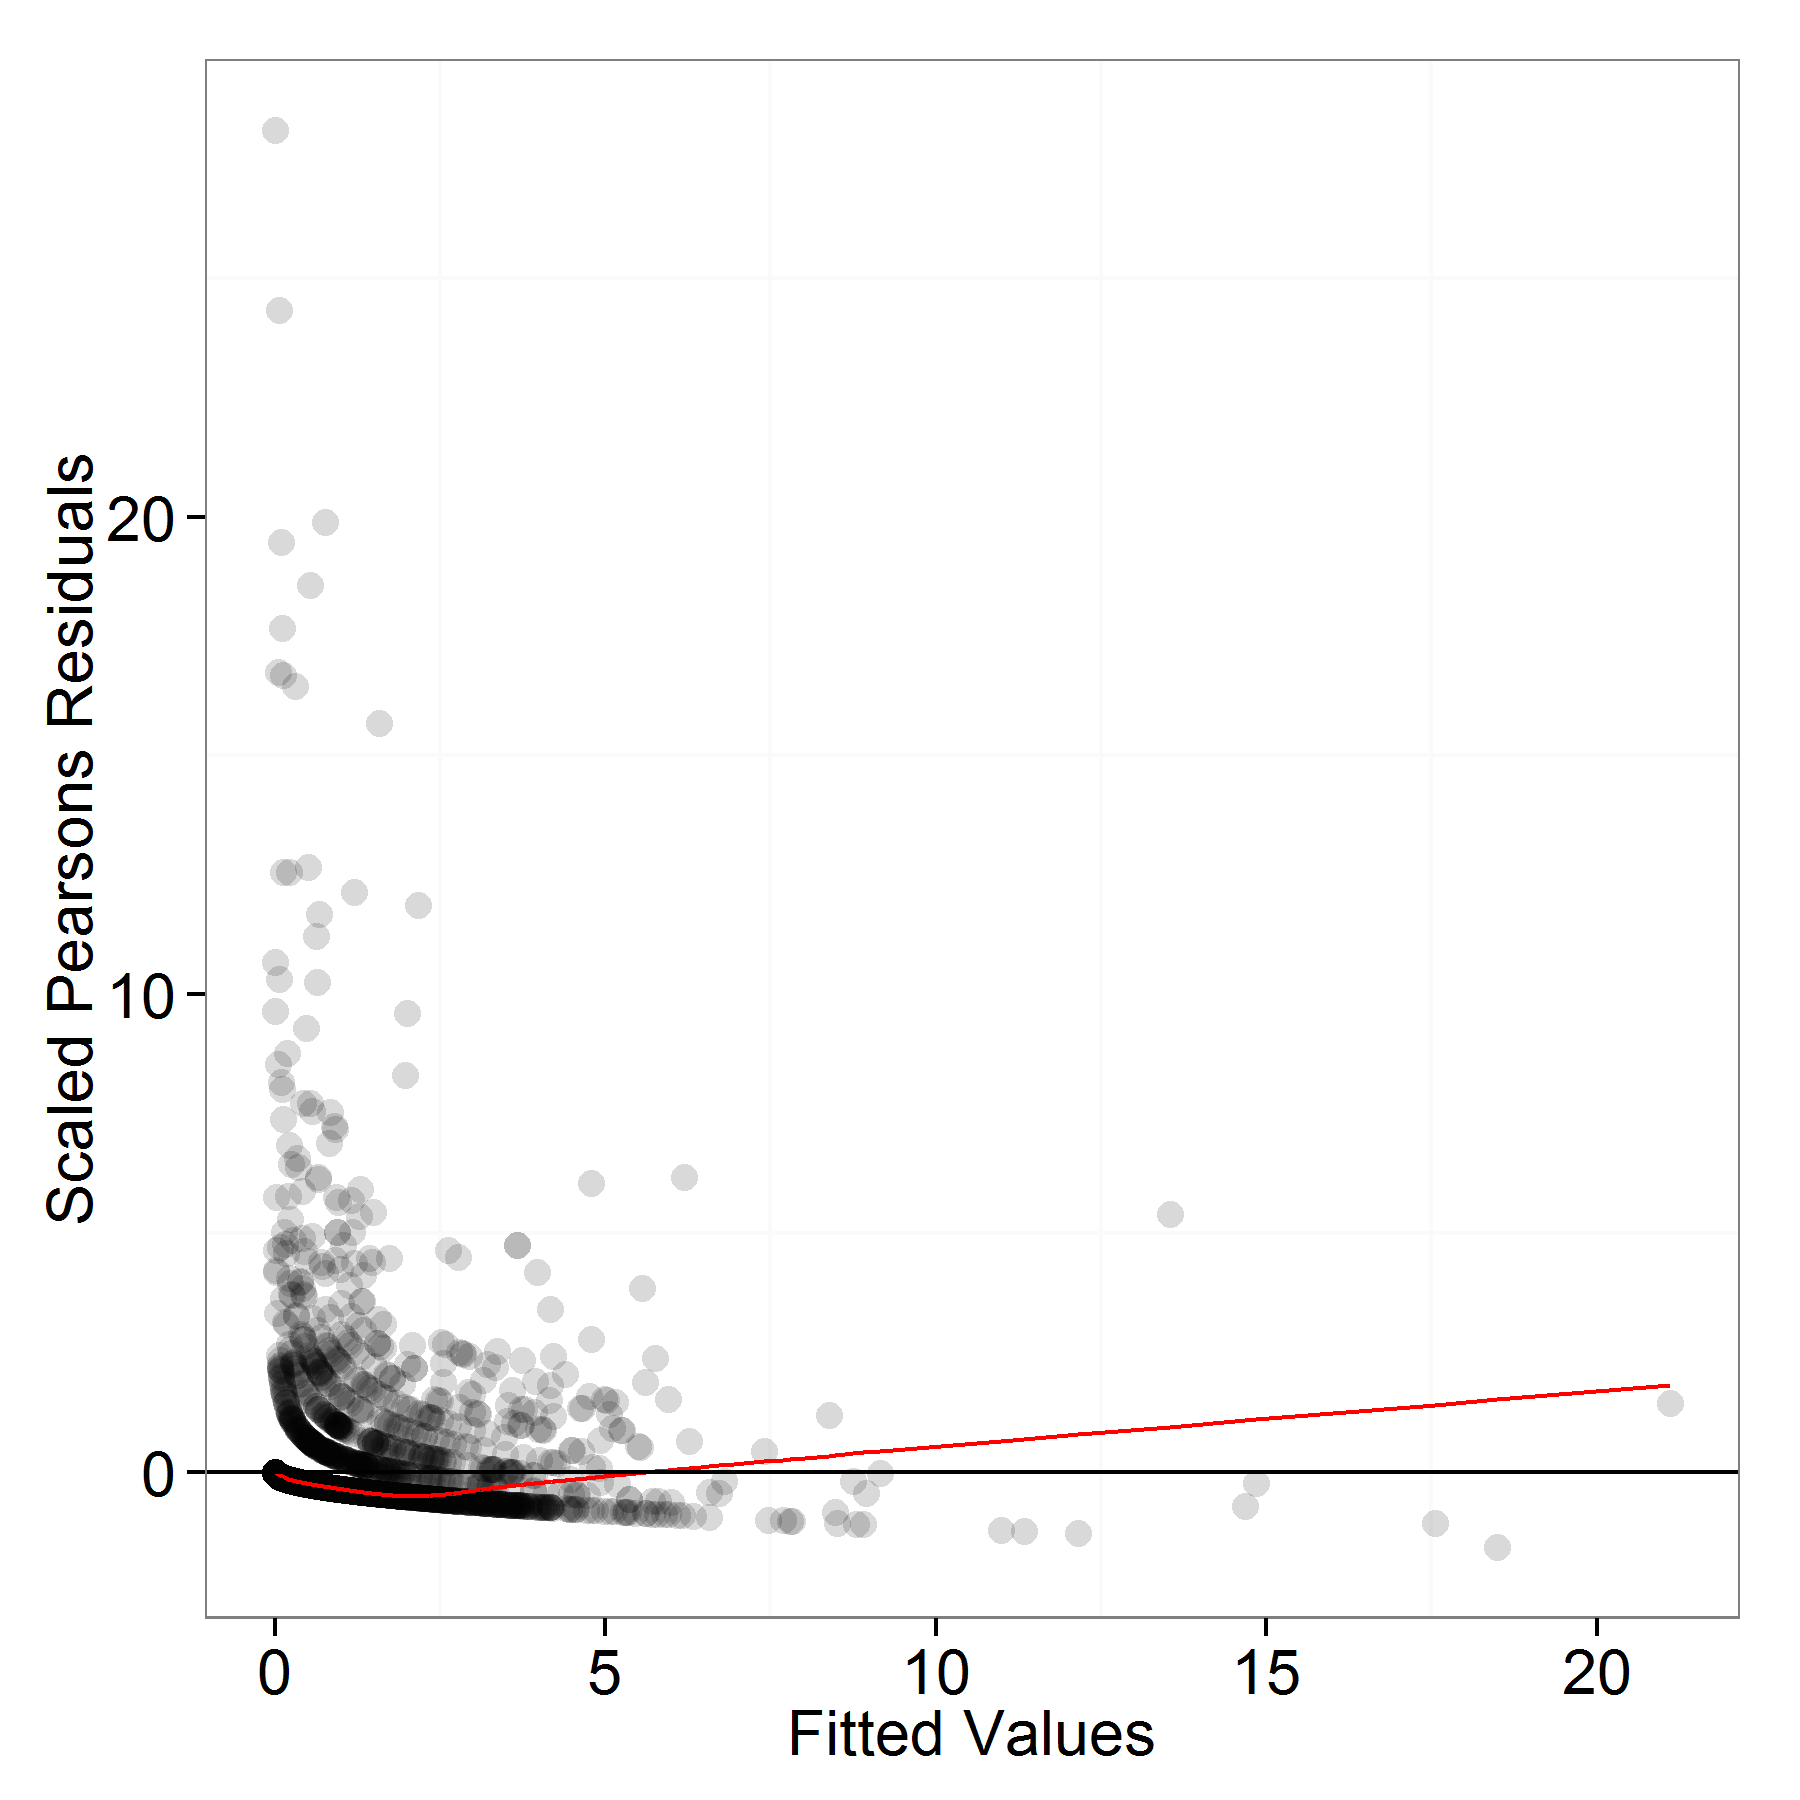
\includegraphics[width=6cm]{FitPlots_resids.png}
  \caption{Diagnostic plot of fitted values vs scaled Pearsons residuals, where the red line is a locally weighted least squares regression to indicate pattern in the plot, which might otherwise be hidden due to over-plotting.}
  \label{fig:diagplots}
\end{figure}
\end{frame}

\begin{frame}
\frametitle{}
\begin{itemize}
\item Possible pattern in residuals but hard to tell due to over-plotting
\item Locally weighted least squares regression line does not indicate an unusual pattern
\pause
\bigskip
\item Conclusion: no issue with model assumption (mean-variance relationship)
\end{itemize}
\end{frame}

%~~~~~~~~~~~~~~~~~~~~~~~~~~~~~~~~~~~~~~~~~~~~~~~~~~
%~~~~~~~~~~~~~~~~~~~~~~~~~~~~~~~~~~~~~~~~~~~~~~~~~~~~~
\subsection{Cumulative Residuals and runs profiles}

\begin{frame}[fragile]
\frametitle{Cumulative residuals and runs profiles}
\begin{itemize}
\item Assessment of systematic over- or under- prediction using cumulative residuals.
\item Assessment of the correlated nature of residuals (how random they are) given that the residuals are ordered by covariate value, predicted value or temporally.
\end{itemize}

\begin{knitrout}\footnotesize
\definecolor{shadecolor}{rgb}{0.969, 0.969, 0.969}\color{fgcolor}\begin{kframe}
\begin{alltt}
\hlfunctioncall{plotCumRes}(geeModel, varlist=\hlfunctioncall{c}(\hlstring{'depth'}), splineParams=splineParams, d2k=dists)
\hlfunctioncall{plotRunsProfile}(geeModel, varlist=\hlfunctioncall{c}(\hlstring{'depth'}))
\end{alltt}
\end{kframe}
\end{knitrout}

\end{frame}

\begin{frame}[fragile]
\frametitle{Cumulative residuals and runs profiles for depth}
\begin{figure}[h]
  \centering
\subfloat[]{
  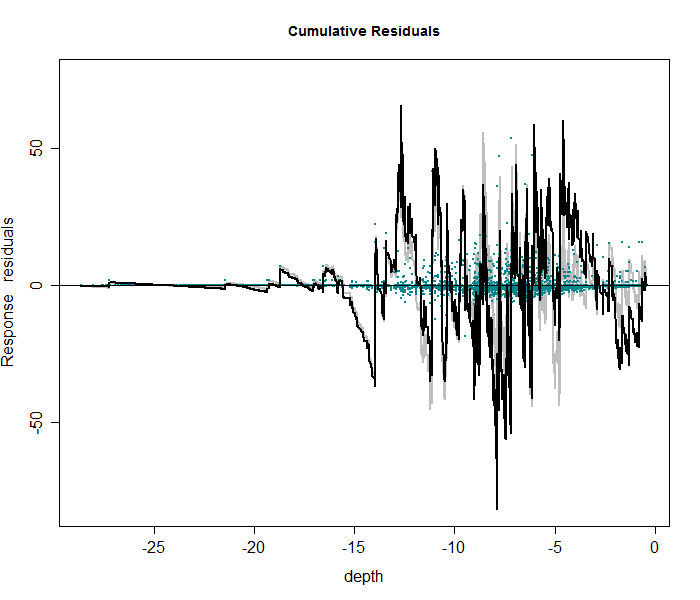
\includegraphics[width=6cm]{CumRes_depth_gee.png}
}
\subfloat[]{
	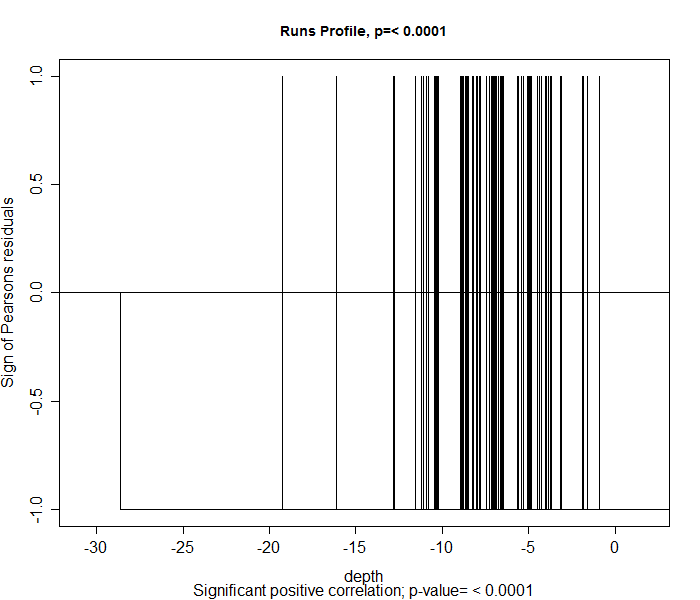
\includegraphics[width=6cm]{RunsProfile_depth_gee.png}
}
    \caption{Cumulative residual plot (a) and runs profile (b) for residuals ordered by depth. The blue points are the residual values, the black line represents the cumulative residuals. The grey line in the background is what we would expect the cumulative residuals to be if depth was modelled correctly.}
  \label{fig:geeruns1}
\end{figure}
\end{frame}

\begin{frame}[fragile]
\frametitle{}
Ordered by \textbf{depth}
\begin{itemize}
\item No systematic over or under prediction
\item Variable modelled appropriately (similar to expected (grey line) and better than Figure \ref{fig:cumres1})
\item Fewer runs than would be expected if residuals were random ($p<0.05$)
\item Significant positive correlation between residuals when ordered by depth
\end{itemize}
\end{frame}

\begin{frame}[fragile]
\frametitle{Cumulative residuals and runs profiles ordered by predicted value}
\begin{figure}[h]
  \centering
    \subfloat[]{
  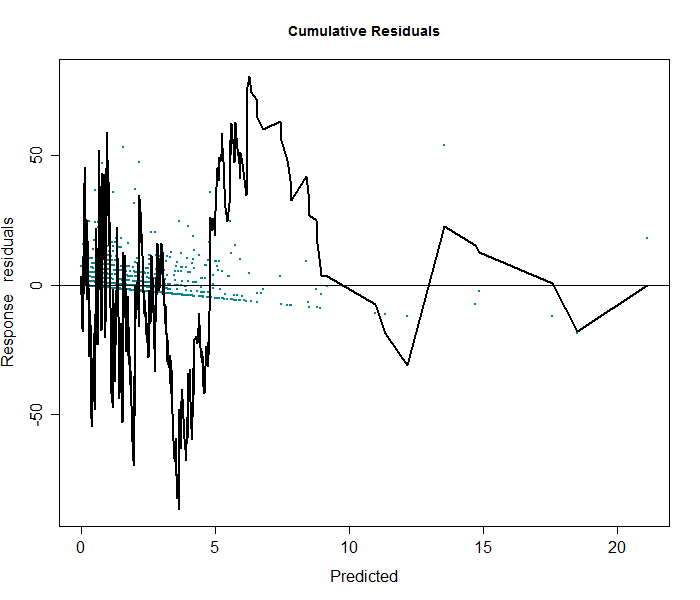
\includegraphics[width=6cm]{CumRes_Predicted_gee.png}
}
\subfloat[]{
	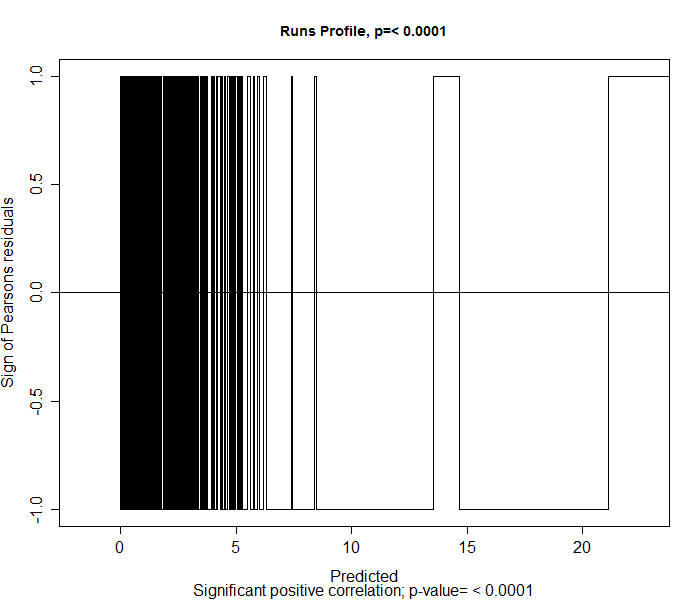
\includegraphics[width=6cm]{RunsProfile_Predicted_gee.png}
}
    \caption{Cumulative residual plot (a) and runs profile (b) for residuals ordered by the predicted value.  The blue points are the residual values and the black line represents the cumulative residuals.}
  \label{fig:geeruns2}
\end{figure}
\end{frame}

\begin{frame}[fragile]
\frametitle{}
Ordered by \textbf{prediction} value
\begin{itemize}
\item Little systematic over or under prediction at predicted counts $< 5$
\item Good mixing at small predicted values
\item But, fewer runs than would be expected if residuals were random ($p<0.05$)
\item Significant positive correlation between residuals when ordered by predicted value
\end{itemize}
\end{frame}

\begin{frame}[fragile]
\frametitle{Cumulative residuals and runs profiles ordered temporally}  
\begin{figure}[h]
  \centering
  \subfloat[]{
  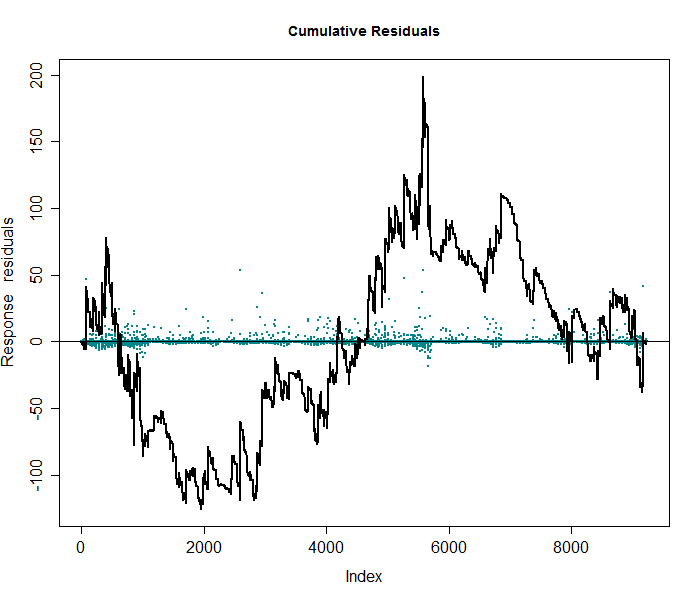
\includegraphics[width=6cm]{CumRes_Index_gee.png}
}
\subfloat[]{
	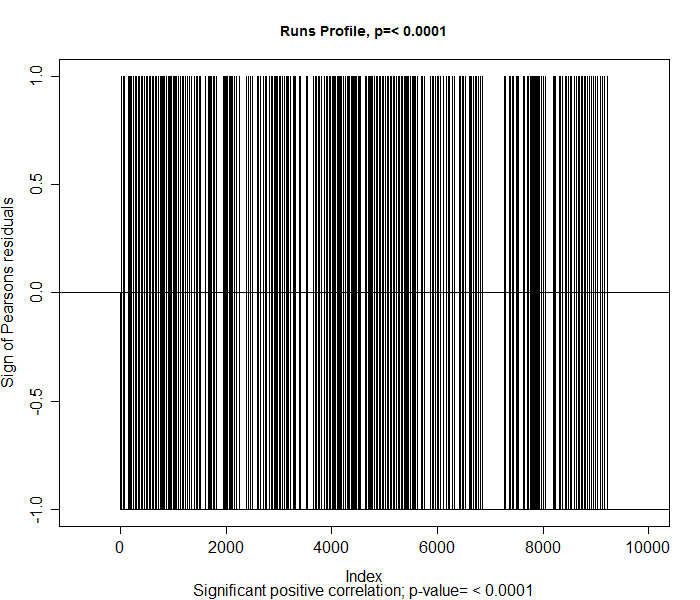
\includegraphics[width=6cm]{RunsProfile_Index_gee.png}
}
  \caption{Cumulative residual plot (a) and runs profile (b) for residuals ordered by the index of observations (temporally).  The blue points are the residual values and the black line represents the cumulative residuals.}
  \label{fig:geeruns3}
\end{figure}
\end{frame}

\begin{frame}[fragile]
\frametitle{}
Ordered by \textbf{index} (temporally)
\begin{itemize}
\item Early observations (before impact) are over predicted and the later (after impact) are under predicted
\item Best mixing of residuals seen in the runs profile 
\item But, still fewer runs than would be expected if residuals were random ($p<0.05$)
\item Significant positive correlation between residuals when ordered temporally
\end{itemize}
\end{frame}

\begin{frame}
\frametitle{Cumulative residuals and runs profiles}
\begin{itemize}
  \item Despite the inclusion of temporal covariates (season and impact) we still have some unmodelled correlation
  \item We have modelled this correlation using GEEs so no need for concern.
  \item $p$-values from ANOVA (used for covariate selection earlier) are reliable due to modelled correlation
\end{itemize}


\end{frame}
% ~~~~~~~~~~~~~~~~~~~~~~~~~~~~~~~~~~~~~~~##
% ~~~~~~~~~~~~~~~~~~~~~~~~~~~~~~~~~~~~~~~##

\subsection{COVRATIO and PRESS statistics}

\begin{frame}[fragile]
\frametitle{}

The PRESS and COVRATIO statistics are relative measures that assess how aspects of the model change when individual blocks are removed from the analysis.

\begin{block}{COVRATIO statistic}
Signals the change in the \textbf{precision of the parameter estimates} when each block is omitted. 
\begin{itemize}
\item Values greater than 1 signal removing the block inflates model standard errors 
\item values less than 1 signal standard errors are smaller when that block is excluded 
\end{itemize}
\end{block}

\begin{block}{PRESS statistic}
Quantifies the sensitivity of \textbf{model predictions} to removing each block. 
\begin{itemize}
\item Relatively large values signal the model is sensitive to these subjects.
\item Model coefficients are re-estimated when each block is omitted (one-by one) and the sum of the squared differences between the response data and the predicted values (when that subject is removed) are found.
\end{itemize}
\end{block}

\pause
\bigskip
\noindent If model predictions or measures of precision appear particularly sensitive to omitted blocks, examine model conclusions based on models with and without the potentially problematic blocks.
\end{frame}

\begin{frame}[fragile]
\frametitle{COVRATIO and PRESS statistics}

\begin{knitrout}\footnotesize
\definecolor{shadecolor}{rgb}{0.969, 0.969, 0.969}\color{fgcolor}\begin{kframe}
\begin{alltt}
\hlfunctioncall{timeInfluenceCheck}(geeModel, count.data$blockid, dists, splineParams)
\end{alltt}
\begin{verbatim}
[1] "Calculating the influence measures will take approximately 7 minutes"
\end{verbatim}
\begin{alltt}
\hlcomment{# influence plots (covratio and press statistics)}
\hlfunctioncall{influence}<-runInfluence(geeModel, count.data$blockid, dists, splineParams)
\end{alltt}
\end{kframe}
\end{knitrout}

\end{frame}

\begin{frame}[fragile]
\frametitle{}
\begin{figure}[h]
  \centering
  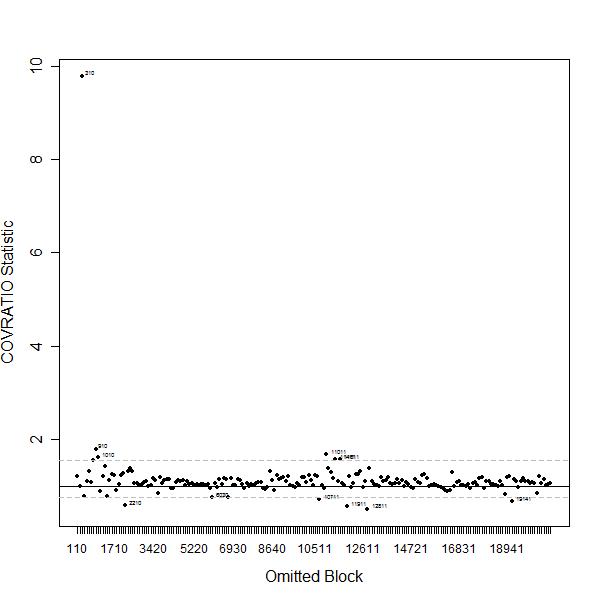
\includegraphics[width=6cm]{InfluenceMeasures_covratio.png}
  \caption{Plot of COVRATIO statistics; the dashed grey lines indicate the lower 2.5\% and upper 97.5\% quantiles of the statistics.}
  \label{fig:influence1}
\end{figure}
\end{frame}

\begin{frame}
\frametitle{COVRATIO statistics}
\begin{itemize}
  \item there will always be blocks outside the dashed lines (they are quantiles)
  \item As it is a relative measure, blocks far away may be of concern
  \item Blocks with COVRATIO statistic $< 1$ are of most concern (decrease in precision when removed) 
  \item Here, block {\tt 310} is far away but results in an increase in standard errors when removed
  \pause
  \bigskip
  \item Conclusion: No issue with blocks unduly influencing the precision of parameter estimates
\end{itemize}
\end{frame}

% ~~~~~~~~~~~~~~~~~~~~~~~~~~~~~~~~~~~~~~~##
% ~~~~~~~~~~~~~~~~~~~~~~~~~~~~~~~~~~~~~~~##
\begin{frame}[fragile]
\frametitle{}
\begin{figure}[h]
  \centering
    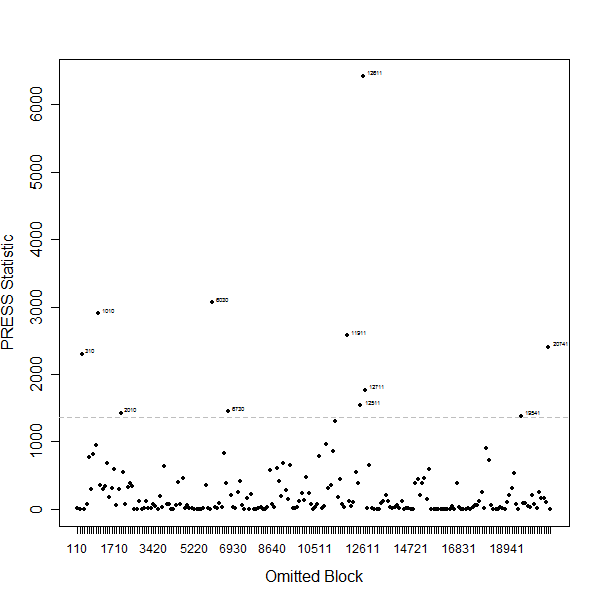
\includegraphics[width=6cm]{InfluenceMeasures_press.png}
  \caption{Plot of PRESS statistics; 95\% of the statistics fall below the dashed grey lines.  Labelled points on both plots are outside the grey dashed line(s) and are labelled with the identifier for the block that has been removed to create the statistic (not an observation number).}
  \label{fig:influence2}
\end{figure}
\end{frame}


\begin{frame}
\frametitle{PRESS statistics}
\begin{itemize}
  \item there will always be blocks above the dashed line (it is a quantile)
  \item As it is a relative measure, blocks far away may be of concern
  \item Here, block {\tt 12611} is far away.  This is the right-hand most transect in season 1 before the impact event and contains only one segment with a bird count.
  \pause
  \bigskip
  \item Conclusion: we may choose to fit a model with and without this block to assess the change in predictions
\end{itemize}
\end{frame}

% ~~~~~~~~~~~~~~~~~~~~~~~~~~~~~~~~~~~~~~~##
% ~~~~~~~~~~~~~~~~~~~~~~~~~~~~~~~~~~~~~~~##
\subsection{Raw Residuals}
\begin{frame}[fragile]
\frametitle{Raw residuals}

Raw residuals (fitted - observed values) can be represented spatially to ascertain if some areas are over/under predicted.  

\begin{itemize}
\item Highest residuals in central area down to right hand side (in cells where birds were detected)
\item No systematic over/under prediction
\bigskip
\item Conclusion: no spatial issue with raw residuals
\end{itemize}
\end{frame}


\begin{frame}[fragile]
\frametitle{Raw residuals}
\begin{figure}[h]
  \centering
  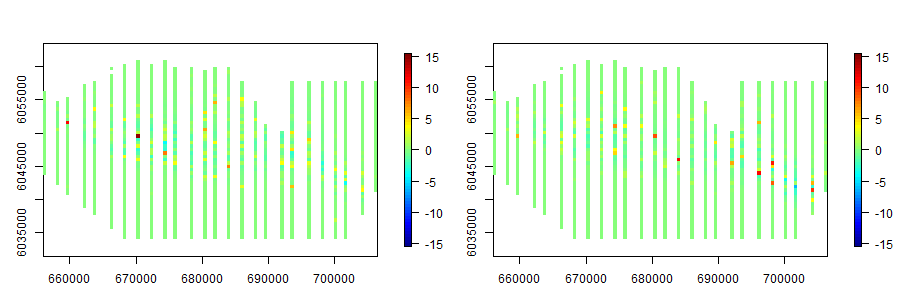
\includegraphics[width=11cm]{residualPlot.png}
  \caption{Raw residuals before impact (left) and after impact (right). These residuals are fitted values - observed values (mean$^*$ birds/km$^2$). * mean density because the predictions for each cell are for each season.}
  \label{fig:rawresid}
\end{figure}
\end{frame}
\begin{frame}[fragile]
\frametitle{}
\begin{knitrout}\footnotesize
\definecolor{shadecolor}{rgb}{0.969, 0.969, 0.969}\color{fgcolor}\begin{kframe}
\begin{alltt}
\hlcomment{# residual plot}
resids <- \hlfunctioncall{fitted}(geeModel) - count.data$NHAT
dims <- \hlfunctioncall{getPlotdimensions}(count.data$x.pos, count.data$y.pos, 
    segmentWidth=500, segmentLength=500)

\hlfunctioncall{par}(mfrow = \hlfunctioncall{c}(1, 2), mar = \hlfunctioncall{c}(3, 3, 3, 5))
\hlfunctioncall{quilt.plot}(count.data$x.pos[count.data$impact == 0], count.data$y.pos[
    count.data$impact == 0], resids[count.data$impact == 0], asp = 1, 
    ncol = dims[2], nrow = dims[1], zlim = \hlfunctioncall{c}(-15.5, 15.5))
\hlfunctioncall{quilt.plot}(count.data$x.pos[count.data$impact == 1], count.data$y.pos[
    count.data$impact == 1], resids[count.data$impact == 1], asp = 1, 
    ncol = dims[2], nrow = dims[1], zlim = \hlfunctioncall{c}(-15.5, 15.5))

\end{alltt}
\end{kframe}
\end{knitrout}
\end{frame}


\begin{frame}
\frametitle{How did we do?}
\begin{table}[h]
%\tiny
\scriptsize
\caption{Table of potential modelling problems, what method was used to assess the problem, was the potential problem an issue in reality and if yes then what was the solution.  Solutions in red were not done and are possibilities for the future.}
\begin{tabular}{l|c|c|c}
\textbf{} & \textbf{Method} & \textbf{Issue (Y/N)} & \textbf{Solution}\\
\hline
Collinearity & VIF & N & -\\
Over-dispersion& - & Y & estimated by GEE\\
Model Fit & Observed vs Fitted & Y & {\color{red} use more covariates}\\
mean-variance relationship & Fitted vs residuals & N & -\\
Correlated Residuals & runs test & Y & modelled by GEE\\
Correlated Residuals & Runs profile & Y & modelled by GEE\\
Covariate specification & cumulative residuals & N & -\\
systematic over/under prediction & cumulative residuals & N & -\\
spatial systematic over/under prediction & raw residual plot & N & -\\
removing blocks & COVRATIO statistics & N & - \\
removing blocks & PRESS statistics & N & - \\
\end{tabular}
\label{tab:fitstats}
\end{table}

\end{frame}
%~~~~~~~~~~~~~~~~~~~~~~~~~~~~~~~~~~~~~~~~~
%~~~~~~~~~~~~~~~~~~~~~~~~~~~~~~~~~~~~~~~~~~~
\section{Prediction and Inference}
\subsection{Data requirements for predicting}
For making predictions, we require a data frame containing grid data with the records we wish to make predictions for. Again, this requires certain columns and records which can be summarised as: \\
\begin{itemize}
\item{\textbf{Columns:} each covariate retained in the best fitting model with exactly matching column names}
\item{\textbf{Columns:} \textit{x.pos} and \textit{y.pos} provide geographic position information used for calculating distance matrices for CReSS/SALSA}
\item{\textbf{Columns:} \textit{area} provides the area of each grid cell.}
\item{\textbf{Rows:} 1 record for each grid cell and for each date and time a prediction is required.}
\end{itemize}

\noindent Using our case study of offshore data, we have a look at our prediction data using the {\tt head} function after we load the data. 
\begin{knitrout}\footnotesize
\definecolor{shadecolor}{rgb}{0.969, 0.969, 0.969}\color{fgcolor}\begin{kframe}
\begin{alltt}
\hlcomment{# If not loaded already, load the prediction grid data}
\hlfunctioncall{data}(predict.data.re)
predictData <- predict.data.re
\hlfunctioncall{head}(predictData)
\end{alltt}
\begin{verbatim}
   area  x.pos   y.pos   depth segment.id season impact   truth
1 0.006 655444 6044450 -27.701          1      1      0 0.001429259
2 0.179 655250 6044750 -28.163          2      1      0 0.051732441
3 0.250 655250 6045250 -28.512          3      1      0 0.084503893
4 0.250 655250 6045750 -28.139          4      1      0 0.069776928
5 0.250 655250 6046250 -27.830          5      1      0 0.059117647
6 0.250 655250 6046750 -27.466          6      1      0 0.048559153
\end{verbatim}
\end{kframe}
\end{knitrout}

\subsection{Making predictions}
\label{ss:predictions}
\noindent We are now going to use these data to make predictions using our best fitting CReSS/Salsa model from the previous sections. This requires three steps: 
\begin{enumerate}
\item{Creating a matrix of distances from prediction data to knots}
\item{Making predictions to the prediction data using the best fitting model}
\item{Converting the predictions back to the response scale}
\end{enumerate}
\begin{knitrout}\footnotesize
\definecolor{shadecolor}{rgb}{0.969, 0.969, 0.969}\color{fgcolor}\begin{kframe}
\begin{alltt}
\hlcomment{# create the distance matrix for predictions }
dists <- \hlfunctioncall{makeDists}(\hlfunctioncall{cbind}(predictData$x.pos, predictData$y.pos), 
    \hlfunctioncall{na.omit}(knotgrid), knotmat = FALSE)$dataDist
\hlcomment{# use baseModel to make predictions to avoid a warning from }
\hlcomment{# using geeModel (same answers though)}
predslink <- \hlfunctioncall{predict}(baseModel, predictData, type = \hlstring{"link"})
\hlcomment{# reversing the log-link to convert predictions back to the response scale}
preds <- \hlfunctioncall{exp}(predslink)
\end{alltt}
\end{kframe}
\end{knitrout}
\noindent The object {\tt preds} contains the predictions for each cell in our prediction grid data. 


\subsection{Visualising the redistribution using predictions}
\noindent We know that our model identified a redistribution of animals within the study area by the significant interaction term between impact and the two-dimensional smooth of \textit{x.pos} and \textit{y.pos}. However, from the model coefficients it is not obvious where the redistribution has occurred. Hence, we are going to investigate this by visualising the redistribution using our predictions. 

\noindent The following is code for plotting the model predictions in Figure \ref{fig:pointest}.
\begin{knitrout}\footnotesize
\definecolor{shadecolor}{rgb}{0.969, 0.969, 0.969}\color{fgcolor}\begin{kframe}
\begin{alltt}
\hlcomment{# plotting the predictions for before and after impact}
\hlfunctioncall{par}(mfrow=c(1,2), mar=c(3,3,3,5))
\hlfunctioncall{quilt.plot}(predictData$x.pos[predictData$impact==0], 
predictData$y.pos[predictData$impact==0], 
preds[predictData$impact==0], asp=1, nrow=104, ncol=54, 
zlim=c(0, maxlim))
\hlfunctioncall{quilt.plot}(predictData$x.pos[predictData$impact==1], 
predictData$y.pos[predictData$impact==1], preds[predictData$impact==1], 
asp=1,nrow=104, ncol=54, zlim=c(0, maxlim))
\end{alltt}
\end{kframe}
\end{knitrout}
\noindent Note: the value for {\tt maxlim} can be determined by plotting both plots without the {\tt zlim} argument first from which you can determine what the maximum value in the scale of either plot is. 
\begin{block}{The {\tt quilt.plot} function}
\begin{itemize}
\item{Plots averages of the predictions for each grid cell}
\item{Subsetting the data using the square brackets restricts the input data to before (left) and after impact (right plot)}
\item{Using the {\tt zlim} argument allows ensuring that left and right plot have the same scale colour scheme}
\end{itemize}
\end{block}

\begin{figure}[h]
  \centering
  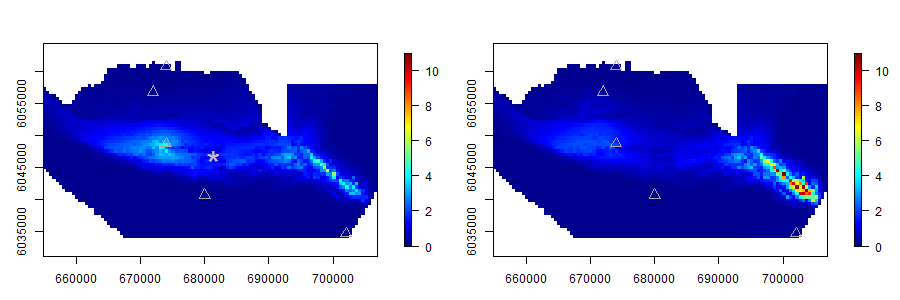
\includegraphics[width=12cm]{pointEstimate.png}
  \caption{Predictions of bird density (mean birds/km$^2$) from the fitted model for before (left) and after (right) an impact event. The * indicated the location of the impact; the $\triangle$ indicate the knot locations. }
  \label{fig:pointest}
\end{figure}

\begin{block}{Conclusion}
\begin{itemize}
  \item Decline in bird density in the central region
  \item Increase in density in the south east of the study area 
  \item The central region is where a known impact has taken place and the results suggest that birds have moved from this region to the south east after the impact event
\end{itemize}
\end{block}

\begin{block}{Next step}
\begin{itemize}
  \item Is this difference real or simply random noise?
  \item We need to classify if the differences are significant or due to sampling variation
  \item We do this by constructing bootstrap confidence intervals for each prediction in the prediction grid data.
\end{itemize}
\end{block}

% ~~~~~~~~~~~~~~~~~~~~~~~~~~~~~~~~~~~~~~~~~~~~~~

\section{Bootstrap Confidence Intervals}
\label{ss:bootstrap}
\noindent Following the predictions from section \ref{ss:predictions}, we now create a set of bootstrap predictions and use these to construct percentile confidence intervals around each prediction from our prediction grid data. We run \textit{B} iterations where for each iteration the following steps are completed: 
\begin{itemize}
\item{resample the original distance data with replacement}
\item{re-fit the detection function to the bootstrapped data and re-estimate the \textit{NHATs} (estimated number of animals)}
\item{re-fit the count model to the bootstrapped data}
\item{using the model coefficients and covariance matrix to sample new coefficients from a multivariate Normal distribution}
\item{make predictions to the study area using these coefficients}
\end{itemize}
\begin{block}{}
This approach incorporates the uncertainty associated with both modelling stages, the detection model and the count model. 
\end{block}

\begin{block}{The {\tt do.bootstrap.cress} function}
This function performs the number of bootstrap iterations specified with the argument \textit{B} where the fitting model for the second stage is CReSS. \\
If a {\tt ddf.obj} is specified, this function automatically applies the 'distance'-approach which includes re-fitting the detection model as described above.\\
Since the prediction object can be quite large, it is not returned but saved into the current working directory. 
\end{block}

\begin{knitrout}\footnotesize
\definecolor{shadecolor}{rgb}{0.969, 0.969, 0.969}\color{fgcolor}\begin{kframe}
\begin{alltt}
\hlcomment{# do the bootstrap}
dis.data$seasonimpact <- \hlfunctioncall{paste}(dis.data$season, dis.data$impact)
\hlfunctioncall{do.bootstrap.cress}(dis.data, predictData, ddf.obj, baseModel, 
    splineParams, dists, resample = \hlstring{"transect.id"}, 
    rename = \hlstring{"segment.id"}, stratum = \hlstring{"seasonimpact"}, B = 250)
\end{alltt}
\end{kframe}
\end{knitrout}

\noindent In the next step we will use these bootstrap predictions to construct our 95\% confidence intervals for each prediction. 

\begin{block}{The {\tt makeBootCIs} function}
Using the {\tt B} bootstrap predictions from a call to the {\tt do.bootstrap.cress} function, the {\tt makeBootCIs} function  creates lower and upper limits for 95\% confidence intervals using the percentile method for each record in the prediction data. \\
\end{block}

\begin{knitrout}\footnotesize
\definecolor{shadecolor}{rgb}{0.969, 0.969, 0.969}\color{fgcolor}\begin{kframe}
\begin{alltt}
\hlcomment{# read in bootstrap predictions}
\hlfunctioncall{load}(predictionboot.RData)
cis <- \hlfunctioncall{makeBootCIs}(bootPreds)
\end{alltt}
\end{kframe}
\end{knitrout}

\pagebreak
\subsection{Visualising Bootstrap Confidence Intervals}
In this section we will investigate whether looking at the lower and upper confidence limits from the 95\% confidence intervals will give us a similar picture as looking at the predictions. 
\begin{figure}[h]
  \centering
  \subfloat{
  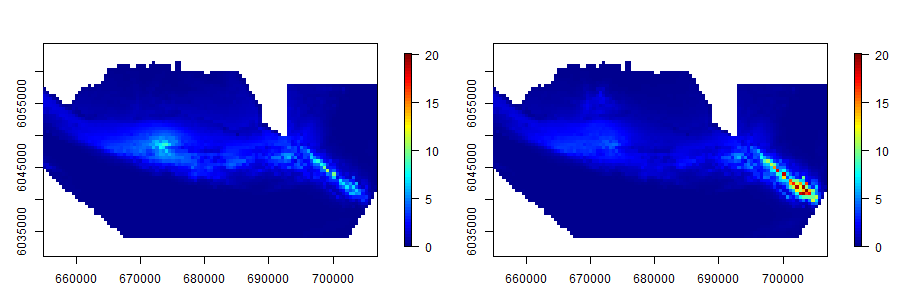
\includegraphics[width=12cm]{cis_upper.png}
  }
  \hfill
  \subfloat{
    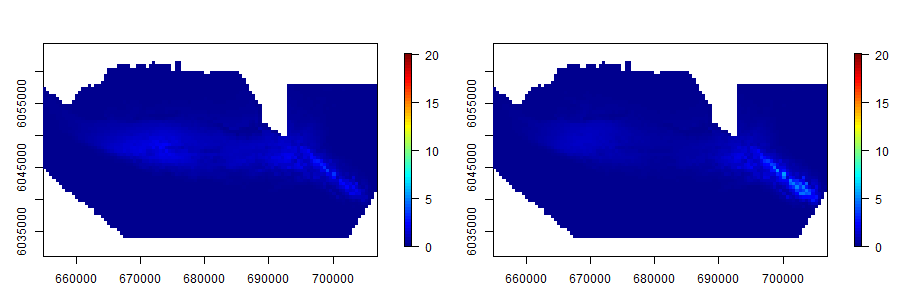
\includegraphics[width=12cm]{cis_lower.png}
  }
  \caption{Upper (top) and lower (bottom) 95\% confidence intervals of bird density (mean birds/km$^2$) from the fitted model from before (left) and after (right) impact.}
  \label{fig:cis}
\end{figure}

\begin{block}{Conclusion}
\begin{itemize}
  \item Lower and upper intervals before impact (left) show a higher density of birds in the central and south east region.  
  \item After impact (right), both lower and upper intervals show a decline in density in the central region and an increase in the area to the south east.  
  \item It is difficult to see where in the study region any significant differences may occur.
\end{itemize}
\end{block}
\begin{block}{Next step}
\begin{itemize}
\item{To see where the redistribution may have occurred we proceed to the next step where we calculate the differences in densities before and after impact for each corresponding pair of predictions.}
\end{itemize}
\end{block}

% ~~~~~~~~~~~~~~~~~~~~~~~~~~~~~~~~~~~~~~~~~~~~~~
% ~~~~~~~~~~~~~~~~~~~~~~~~~~~~~~~~~~~~~~~~~~~~~~
\section{Significant Differences}
\frametitle{}
\noindent In this section we will estimate the differences in predictions for each corresponding pair of records from our prediction grid data. The first half of our prediction grid data consists of records from before impact while the second half consists of records from after impact. \\

\noindent Note that the before and after data need to be ordered in the same manner and of the same length. 


\begin{block}{The {\tt getDifferences} function}
For each bootstrap iteration the differences in predictions from before and after impact are calculated (Density$_{after}$ - Density$_{before}$) and 95\% confidence intervals calculated using the percentile method. \\

\noindent If these intervals contain the value zero, a '0' is recorded. If they do not contain the value zero, '1' is recorded if the lower limit is above zero as an indication that the difference is significantly positive (increase in animal densities after impact). A '-1' is recorded if the upper limit is below zero, indicating that the difference is significantly negative (decrease in animal densities after impact). \\

\noindent The function returns a list of two objects: 
\begin{itemize}
\item{The median for each difference}
\item{The marker for significant positive and negative differences}
\end{itemize}
\end{block}


\begin{knitrout}\footnotesize
\definecolor{shadecolor}{rgb}{0.969, 0.969, 0.969}\color{fgcolor}\begin{kframe}
\begin{alltt}
differences <- \hlfunctioncall{getDifferences}(beforePreds = 
        bootPreds[predictData$impact == 0, ], 
        afterPreds = bootPreds[predictData$impact == 1, ])
\end{alltt}
\begin{verbatim}
NOTE: 1 bootstrap(s) removed due to infinite values
\end{verbatim}
\end{kframe}
\end{knitrout}


\subsection{Visualising significant differences}
To illustrate the differences in animal densities after impact, we plot the calculated differences (Density$_{after}$ - Density$_{before}$) using the {\tt quilt.plot} function.\\

\noindent The locations of the significant differences are added to the same plot using the '$\circ$' and '+' symbols. 

\begin{knitrout}\footnotesize
\definecolor{shadecolor}{rgb}{0.969, 0.969, 0.969}\color{fgcolor}\begin{kframe}
\begin{alltt}
\hlcomment{# The median for each after - before difference}
meandiff <- differences$meandiff
\hlcomment{# The marker for each after - before difference: }
\hlcomment{# positive ('1') and negative ('-') significant differences}
marker <- differences$significanceMarker
\hlfunctioncall{par}(mfrow = \hlfunctioncall{c}(1, 1))
\hlfunctioncall{quilt.plot}(predictData$x.pos[predictData$impact == 0], 
predictData$y.pos[predictData$impact ==  0], 
meandiff, asp = 1, nrow = 104, ncol = 55)
\hlcomment{# add + or - depending on significance of cells.  Just}
\hlcomment{# requires one significance out of all to be allocated}
\hlfunctioncall{points}(predictData$x.pos[predictData$impact == 0][marker == 1], 
    predictData$y.pos[predictData$impact == 0][marker == 1], 
    pch = \hlstring{"+"}, col = \hlstring{"darkgrey"}, cex = 0.75)
\hlfunctioncall{points}(predictData$x.pos[predictData$impact == 0][marker == (-1)], 
    predictData$y.pos[predictData$impact == 0][marker == (-1)], 
    col = \hlstring{"darkgrey"}, cex = 0.75)
\hlfunctioncall{points}(681417.3, 6046910, cex = 3, pch = \hlstring{"*"}, lwd = 1, col = \hlstring{"grey"})
\end{alltt}
\end{kframe}
\end{knitrout}

\begin{figure}[h]
  \centering
  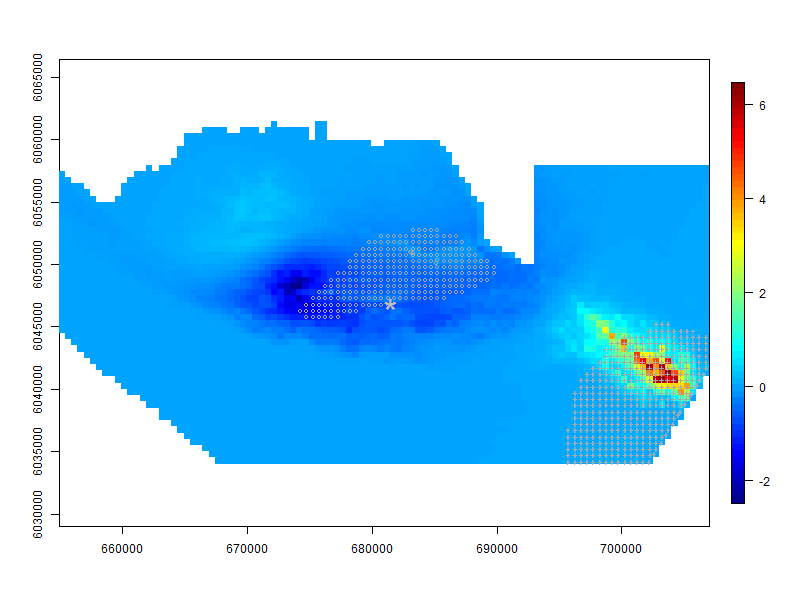
\includegraphics[width=10cm]{differencePlot.png}
  \tiny
  \caption{Mean differences in predicted bird density (mean birds/km$^2$) before and after impact.  Positive values indicate more birds post impact and negative values fewer birds post impact.  Significant differences were calculated using percentile confidence intervals: '+' indicates a significant positive difference and '-' a significant negative one.  The grey star is the site of the impact event.}
  \label{fig:diffs}
\end{figure}

\begin{block}{Conclusion}
 \begin{itemize}
  \item There was a significant decline in animals around the impact site and in the North of the study area
  \item There was also a significant increase in animals in the south east of the study area
\end{itemize}
\end{block}

% ~~~~~~~~~~~~~~~~~~~~~~~~~~~~~~~~~~~~~~~~~~~~~~
% ~~~~~~~~~~~~~~~~~~~~~~~~~~~~~~~~~~~~~~~~~~~~~~

\section{Comparison to the Truth}
Here we will finalise our analysis by comparing our results with the truth. This is possible as our data was simulated and hence the parameter values known. \\
\subsection{Detection function}
We created detections from a half-normal detection function with a known scale parameter. Our model selection procedure identified the half-normal model as the one with the best fit. 
\begin{table}[h]
\begin{tabular}{l|c|c|c}
 & \textbf{True value} & \textbf{Maximum likelihood} & \textbf{95\% CI} \\
 & & \textbf{estimate} & \\
\hline
{Scale parameter}& 120 & 116.1  &(112.7, 122.4)\\
\end{tabular}
\end{table}
\begin{block}{Conclusion}
\begin{itemize}
\item{We were able to identify the type of model correctly} 
\item{Our best guess of the true value for the scale parameter based on the data was 116.1. }
\item{We were 95\% sure the true scale parameter for the half-normal detection function was between 112.7 and 122.4. The true value for this parameter was captured by this interval.}
\end{itemize}
\end{block}

\subsection{Overdispersion and correlation}
We created data that were both overdispersed and positively correlated within any {\tt transect.id} (i.e. observed detections from the same transect repeat). 

\begin{table}[ht]
\centering
\begin{tabular}{l|r}
\textbf{Truth} & \textbf{Model}\\
\hline
Overdispersed  data & estimated overdispersion \\
 & parameter was greater than 1\\
\hline
Positively correlated data & accounted for using\\
 & GEE-based \textit{p}-values\\
\end{tabular}\end{table}

\begin{block}{Conclusion}
We conclude that our proposed methods are capable of identifying overdispersion and correlation in the data.
\end{block}

\subsection{Type of impact}
For this particular data set, the total number of animals before and after impact did not change. The type of impact that we implemented was a redistribution from the area surrounding the impact into the south east of the study area. 

\begin{table}[ht]
\centering
\begin{tabular}{l|r}
\textbf{Truth} & \textbf{Our model}\\
\hline
Redistribution  & identified with a \\
within study area & significant interaction term\\
\hline
Overall abundance  & identified with the non-significant \\
remained the same & main effect for impact\\
\end{tabular}
\end{table}

\begin{block}{Conclusion}
We conclude that our model was capable of correctly identifying the redistribution effect and removed and reallocated birds to the correct locations despite highly correlated and overdispersed data.\\
\end{block}



%\end{document}
